%%%%%%%%%%%%%%%%%%%%%%%%%%%%%%%%%%%%%%%%%%%%%%%%%%%%%%%%%%%%%%%%%%%%%%%%%%%%
% AGUJournalTemplate.tex: this template file is for articles formatted with LaTeX
%
% This file includes commands and instructions
% given in the order necessary to produce a final output that will
% satisfy AGU requirements, including customized APA reference formatting.
%
% You may copy this file and give it your
% article name, and enter your text.
%
%
% Step 1: Set the \documentclass
%
%

%% To submit your paper:
\documentclass[draft]{agujournal2019}
\usepackage{url} %this package should fix any errors with URLs in refs.
\usepackage{lineno}
\usepackage[inline]{trackchanges} %for better track changes. finalnew option will compile document with changes incorporated.
\usepackage{soul}
\usepackage{amsmath}
\linenumbers
%%%%%%%
% As of 2018 we recommend use of the TrackChanges package to mark revisions.
% The trackchanges package adds five new LaTeX commands:
%
%  \note[editor]{The note}
%  \annote[editor]{Text to annotate}{The note}
%  \add[editor]{Text to add}
%  \remove[editor]{Text to remove}
%  \change[editor]{Text to remove}{Text to add}
%
% complete documentation is here: http://trackchanges.sourceforge.net/
%%%%%%%

\draftfalse

%% Enter journal name below.
%% Choose from this list of Journals:
%
% JGR: Atmospheres
% JGR: Biogeosciences
% JGR: Earth Surface
% JGR: Oceans
% JGR: Planets
% JGR: Solid Earth
% JGR: Space Physics
% Global Biogeochemical Cycles
% Geophysical Research Letters
% Paleoceanography and Paleoclimatology
% Radio Science
% Reviews of Geophysics
% Tectonics
% Space Weather
% Water Resources Research
% Geochemistry, Geophysics, Geosystems
% Journal of Advances in Modeling Earth Systems (JAMES)
% Earth's Future
% Earth and Space Science
% Geohealth
%
% ie, \journalname{Water Resources Research}

\journalname{Journal of Advances in Modeling Earth Systems (JAMES)}


\begin{document}

%% ------------------------------------------------------------------------ %%
%  Title
%
% (A title should be specific, informative, and brief. Use
% abbreviations only if they are defined in the abstract. Titles that
% start with general keywords then specific terms are optimized in
% searches)
%
%% ------------------------------------------------------------------------ %%

% Example: \title{This is a test title}

\title{Design and implementation of a data-driven parameterization for mesoscale eddy-induced transport: idealized two-layer configurations}

%% ------------------------------------------------------------------------ %%
%
%  AUTHORS AND AFFILIATIONS
%
%% ------------------------------------------------------------------------ %%

% Authors are individuals who have significantly contributed to the
% research and preparation of the article. Group authors are allowed, if
% each author in the group is separately identified in an appendix.)

% List authors by first name or initial followed by last name and
% separated by commas. Use \affil{} to number affiliations, and
% \thanks{} for author notes.
% Additional author notes should be indicated with \thanks{} (for
% example, for current addresses).

% Example: \authors{A. B. Author\affil{1}\thanks{Current address, Antartica}, B. C. Author\affil{2,3}, and D. E.
% Author\affil{3,4}\thanks{Also funded by Monsanto.}}

\authors{Dhruv Balwada\affil{1}, 
Pavel Perezhogin\affil{2}, 
%Ryan Abernathey\affil{4}, 
Alistair Adcroft\affil{3}, 
and Laure Zanna\affil{2,4}}  


% \affiliation{1}{First Affiliation}
% \affiliation{2}{Second Affiliation}
% \affiliation{3}{Third Affiliation}
% \affiliation{4}{Fourth Affiliation}

\affiliation{1}{Lamont-Doherty Earth Observatory, Columbia University, Palisades, NY, USA}
\affiliation{2}{Courant Institute of Mathematical Science, New York University, New York, NY, USA}
\affiliation{3}{Princeton University, Princeton, NJ, USA}
\affiliation{4}{Center for Data Science, New York University, New York, NY, USA}



%(repeat as many times as is necessary)

%% Corresponding Author:
% Corresponding author mailing address and e-mail address:

% (include name and email addresses of the corresponding author.  More
% than one corresponding author is allowed in this LaTeX file and for
% publication; but only one corresponding author is allowed in our
% editorial system.)

% Example: \correspondingauthor{First and Last Name}{email@address.edu}

\correspondingauthor{Dhruv Balwada}{dbalwada@ldeo.columbia.edu}

%% Keypoints, final entry on title page.

%  List up to three key points (at least one is required)
%  Key Points summarize the main points and conclusions of the article
%  Each must be 140 characters or fewer with no special characters or punctuation and must be complete sentences

% Example:
% \begin{keypoints}
% \item	List up to three key points (at least one is required)
% \item	Key Points summarize the main points and conclusions of the article
% \item	Each must be 140 characters or fewer with no special characters or punctuation and must be complete sentences
% \end{keypoints}

\begin{keypoints}
\item A data-driven parameterization for mesoscale eddy-induced transport is developed, and implemented in NOAA GFDL's MOM6
\item This parameterization replaces the diffusive closure in traditional Gent-McWilliams scheme with an ANN 
\item In 2 layer simulations the parameterization reduces potential energy without overly dissipating the kinetic energy
\end{keypoints}

%% ------------------------------------------------------------------------ %%
%
%  ABSTRACT and PLAIN LANGUAGE SUMMARY
%
% A good Abstract will begin with a short description of the problem
% being addressed, briefly describe the new data or analyses, then
% briefly states the main conclusion(s) and how they are supported and
% uncertainties.

% The Plain Language Summary should be written for a broad audience,
% including journalists and the science-interested public, that will not have 
% a background in your field.
%
% A Plain Language Summary is required in GRL, JGR: Planets, JGR: Biogeosciences,
% JGR: Oceans, G-Cubed, Reviews of Geophysics, and JAMES.
% see http://sharingscience.agu.org/creating-plain-language-summary/)
%
%% ------------------------------------------------------------------------ %%

%% \begin{abstract} starts the second page

\begin{abstract}
Mesoscale eddies contribute to ocean transport and are a major sink of available potential energy (APE). When these eddies are not resolved or only partially resolved in a model, their effects need to be parameterized to simulate a realistic large-scale state. Traditionally, this is achieved via the Gent-McWilliams (GM) parameterization, which represents the eddy-induced transport in terms of a downgradient diffusion. While effective at capturing the bulk APE removal by eddies, the downgradient diffusive framework limits the structural accuracy of the parameterized fluxes, which in reality can contain significant upgradient and cross-gradient components. Additionally, at eddy permitting resolutions, GM can negatively impact the resolved eddies, and is often turned off in regions where eddies are partially resolved. Here we present a novel data-driven parameterization that is not constrained to be diffusive, and can capture the full structure of the eddy-induced fluxes while extracting APE and without overly negative impacts on the resolved flow. It is both flow-aware and scale-aware, and its magnitude can be tuned using an O(1) non-dimensional number.
Features like non-dimensional inputs/outputs, lateral non-locality, flow-dependent coordinates, and range limitation improve the generalization of the data-driven scheme. A small neural network is used, ensuring low cost and ease of implementation.
The parameterization performs skillfully in offline evaluation, especially at scales smaller than the largest eddies. It is implemented in NOAA GFDL$'$s MOM6 and shown to be skillful in online tests in two-layer idealized simulations of a zonal channel and a wind-driven gyre, at both eddy-permitting and non-eddying resolutions.
\end{abstract}

\section*{Plain Language Summary}
Mesoscale ($\sim$100~km) eddies are the dominant flows in the ocean and play a key role in shaping large-scale circulation features such as wind-driven gyres and the meridional overturning circulation. Since these eddies are not fully resolved in many  ocean models -- especially those that are run for long periods or including many ensemble members -- their effects must be represented through parameterizations. 

We present a new data-driven parameterization designed to better represent mesoscale eddy effects in ocean models. The parameterization is trained using data from a high-resolution simulations, and is formed of a small neural network that is designed to be flow-aware, scale-aware, and computationally efficient. The parameterization is implemented in the MOM6 ocean model and shows skillful performance both offline and online in idealized simulations. It extracts APE from large scale flow without degrading resolved features, offering a promising enhancement to the existing Gent-McWilliams (GM) parameterization.

%% ------------------------------------------------------------------------ %%
%
%  TEXT
%
%% ------------------------------------------------------------------------ %%

%%% Suggested section heads:
\section{Introduction}
% Big problem in science 
Ocean circulation models solve equations describing the motions in the ocean on a finite-size discrete grid, and are thus unable to resolve the phenomena at scales smaller than the grid scales. However, it is often the case that these sub-grid phenomena are more than just small-scale variability, and have a profound impact on the characteristics of the resolved motions. To ensure fidelity of the model behavior at the resolved scales, the effects of these sub-grid phenomena need to be appropriately parameterized. An important and often unresolved or partially resolved range of scales in ocean models are the mesoscales. 

%Oceanic flows are replete with mesoscale eddies (scales of $\sim50-200$km). 
Mesoscales ($\sim50-200$km) are the dominant energy-containing scales in the ocean \cite{ferrari2009ocean}, playing an important role in shaping the mean circulation and stratification \cite{gent2011gent}, and in transporting tracers \cite{meredith2021ocean}. These eddies are believed to be largely generated as a result of baroclinic instability \cite{killworth1997parameterization, smith2007geography}, which has its fastest growth rate at scales close to the first baroclinic deformation radius (scales of $\sim10-100$km) \cite{chelton1998geographical, tulloch2011scales}. Also, these instabilities have a tendency to grow at the expense of the available potential energy (APE), and thus a bulk effect is to flatten isopycnals in the ocean. The dominance of rotation effects at these scales also usually leads to a subsequent inverse kinetic energy (KE) cascade, which is why the dominant peak of KE is usually larger than the dominant scale of the instability \cite{tulloch2011scales}. 
Thus, to properly resolve these eddies and their effects the model grid spacing needs to be smaller than the deformation radius \cite{hallberg2013using}. The inverse cascade also takes place in the vertical \cite{smith2002scales}, transferring energy to the barotropic and first couple of baroclinic modes, and the associated flows tend to have weak vertical shear and do not generate small-scale turbulence or diapycnal mixing --- mesoscale flow is predominantly adiabatic in the ocean interior. 


% Narrower problem within
Conventionally, mesoscale eddy effects have been parameterized using the Gent-McWilliams (GM) parameterization \cite{gent1990isopycnal}, particularly in models that do not resolve the deformation radius. The GM parameterization was designed to respect two important aspects of mesoscale processes: (i) the parameterization is adiabatic, and (ii) the net effect of the parameterization is to reduce APE. 
%In models with depth as the vertical coordinate, this is achieved by representing the horizontal eddy fluxes in the form of a horizontally downgradient buoyancy diffusion and then setting the vertical component of the eddy flux such that the net flux is along isopycnals and the resulting operator behaves like advection. In practice this is achieved by defining an eddy-induced stream function, which is set using the parameterized horizontal eddy buoyancy fluxes. 
%In isopycnal models, the mesoscale eddy effects are parameterized by diffusing the interface heights, which is also usually represented as extra eddy-induced advection or a streamfunction. 
In both depth-coordinate and isopycnal models, the mesoscale eddy effects are represented as an eddy-induced advection defined through a streamfunction. In depth-coordinate models, this streamfunction is constructed from downgradient diffusion of horizontal eddy buoyancy fluxes, while in isopycnal models it arises from a diffusion of interface heights.
The GM parameterization has led to dramatic improvements in the ocean simulations, the adiabatic aspect ensures that water masses were not eroded away in the interior by spurious diffusion. However, the choice of isotropic diffusion as a closure and the associated eddy diffusivity has always been a major source of uncertainty and is an active area of research. 


%\cite<e.g.>[]{visbeck1997specification, ferreira2005estimating, eden2008towards, marshall2012framework, jansen2015parameterization}. Also, as with all conventional ocean parameterizations, this scheme was designed to represent the bulk effects of eddies and not to have any skill in representing the spatial or temporal structures of the eddy effects, which leads to detrimental effects at resolutions where eddies are partially resolved \cite{hallberg2013using, mak2023scale}.

Since the original work of \citeA{gent1990isopycnal}, research has advanced along several fronts: improved estimation of eddy diffusivity, extensions of the diffusive operator itself, and complementary approaches that address processes GM does not represent. 
Observations, models, and theory all indicate that the 
eddy diffusivity must vary in space and time 
\cite<e.g.>[]{ferreira2005estimating, kusters2025global}, motivating approaches based on mixing-length arguments \cite{visbeck1997specification, eden2008towards}, linear stability analysis \cite{eden2012implementing, eden2025rossmix}, and energy-budget constraints from the MEKE \cite{jansen2015parameterization, jansen2019toward} and GEOMETRIC \cite{marshall2012framework, mak2018implementation} closures. 
The GM operator itself has also been extended: \citeA{smith2004anisotropic} introduced an anisotropic formulation, and \citeA{eden2023simple} showed that biharmonic PV mixing is equivalent to biharmonic friction plus biharmonic thickness mixing, providing a form of GM appropriate for eddy-permitting models. A separate but related challenge is that GM, by design, removes APE without returning any KE to the resolved flow, leaving coarse models under-energized. This has motivated backscatter parameterizations that couple energy return through the momentum equations, either deterministically \cite{bachman2019gm+, jansen2019toward} or stochastically \cite{grooms2025stochastic}. At eddy-permitting resolutions, standard GM is known to excessively damp the partially resolved eddies \cite{hallberg2013using}, which has led to the use of resolution functions to taper or disable GM \cite{hallberg2013using, adcroft2019gfdl}, as well as the proposal by \citeA{mak2023scale} to apply GM only to the large-scale field via a splitting approach. These advances have substantially improved the physical realism of the conventional diffusive closure in GM. However, all remain rooted in the assumption of downgradient diffusion, which limits the structural accuracy of the predicted fluxes — the eddy fluxes diagnosed from high-resolution simulations contain significant upgradient and cross-gradient components that cannot be captured by a diffusive operator \cite<e.g.>[]{bachman2020diagnosis, kamenkovich2021complexity, uchida2023cautionary}. More broadly, most of these approaches do not fully leverage the information available in high-resolution simulations to move beyond the diffusive framework.

% Evaluation of a scalar eddy transport coefficient based on geometric constraints, Bachman 2017 gives a nice concise overview of some methods to approximate the eddy diff. 

In recent years, machine learning (ML) based methods have started to show a lot of promise in improving different aspects of computational modeling, including improving parameterizations \cite{bracco2025machine, lai2024machine}. While conventional parameterizations require domain scientists to develop mathematical operators, e.g. isotropic diffusion or biharmonic friction, that are at best able to mimic the bulk effects of sub-grid phenomena, ML methods directly learn the numerical mapping between the sub-grid effects and the large-scale fields using appropriate data. It is also possible to design ML models to obey physical properties through modifications to the architectural design or the loss function \cite{beucler2021enforcing, zanna2020data}. These methods have led to the development of parameterizations for idealized models \cite{ross2023benchmarking, srinivasan2023turbulence}, thermodynamic and momentum tendencies in the atmosphere \cite{brenowitz2018prognostic, yuval2021use}, boundary layers processes in the ocean \cite{sane2023parameterizing, ramadhan2020capturing, bodner2023data}, and momentum tendencies in the ocean \cite{zhang2023implementation, zanna2020data, perezhogin2024stable}. Many of these new parameterizations have demonstrated improvements over conventional parameterizations in various metrics, including offline prediction accuracy, reduced biases in mean state and variability, and improved energy spectra in online simulations, though the specific baselines and metrics vary across studies. The potential issues with implementation, stability and generalization remain an area of rapidly evolving research \cite{zanna2025framework}.  
While many sub-grid effects of ocean eddies have been investigated using this approach, the impact of mesoscale eddies on the density or thickness field - the aspect parameterized by the GM parameterization - has not yet been addressed using data-driven parameterizations. 

% Summary
Here we present a new data-driven parameterization to account for the impact that mesoscale eddies have on the thickness or density field in the ocean. Our parameterization is designed to ensure that it maintains the important adiabatic constraint that was introduced by the GM parameterization, and is thus framed as an eddy-induced transport in terms of a stream function. However, unlike GM, our parameterization does not rely on diffusion and is not designed to be a local sink of APE; rather it is optimized to accurately capture the pointwise patterns of the eddy-induced fluxes, including their magnitude and direction, which can locally be upgradient or cross-gradient relative to the large-scale density fields. With an eye towards implementation, we use a small artificial neural network (ANN), which can be easily added to any ocean model code. We implemented this ANN into GFDL's Modular Ocean Model 6 (MOM6), and show its effects in idealized two-layer simulations where mesoscale eddies are the dominant turbulent process. In a follow up study, we will extend this work to a heirarchy of more realistic simulations.
In section 2 we describe the filtering framework that is used to diagnose the sub-grid impact of eddies from high-resolution simulations, and in section 3 describe how to cast these sub-grid effects into a numerical mapping that potentially has some ability to generalize to unseen data. Also, in section 3 we describe the ML architecture, and training process. 
In section 4 we describe the high-resolution datasets and how they were processed. In section 5 we show that our parameterization is successful in both offline and online tests, and finally, in section 6 we conclude with a discussion, potential caveats and an outlook towards future work. 


\section{Sub-grid thickness fluxes}
%Ocean circulation and turbulence is a specialized example of a rotating stratified fluid, which is primarily forced by winds, tides and surface buoyancy fluxes; and shaped by bathymetric features. When modeling this flow, particularly from the perspective of mesoscale eddies and their adiabatic effects in the interior, it is often convenient to cast the equations in terms of isopycnal layered equations. Thus, here we present the formulation for layered coordinates, and a complementary formulation for z-coordinates in presented in the appendix. 
The mesoscale processes can be most strictly isolated with the help of an isopycnal model, as the adiabatic and diabatic processes are clearly distinguished in this framework.
In this framework (stacked shallow water or isopycnal coordinate) the flow can be modeled using momentum and thickness equations \cite<e.g.>{vallis2017atmospheric, loose2023comparing}. The thickness equation, the primary focus of our study, can be written for each layer as, 
\begin{linenomath*}
\begin{equation}
    \partial_t h_n + \nabla \cdot (\mathbf{u}_n h_n) = 0,
\end{equation}
\end{linenomath*}
where $h_n$ and $\mathbf{u}_n = (u_n, v_n)$ are the thickness and velocity in the $n^{th}$ layer respectively.%$Q$ corresponds to diabatic sources or sinks. 

These equations can simulate the flow over the full spectrum of scales where its assumptions are valid, but with a finite grid size only a limited range of scales can be resolved. Here we distinguish between scales that can be resolved and that are too small to be resolved (sub-grid)
using a combination of spatial filtering and coarse-graining $\overline{(\cdot)}$, as is routinely done in the large eddy simulation (LES) framework \cite{sagaut2005large, aluie2018mapping}. The high-pass signal after applying this spatial operation is referred to as \textit{sub-grid} flows in this study.
Consequently, the impact of sub-grid flow, on the resolved flows, can be elucidated in the $n^{th}$ layer thickness equation as,
\begin{linenomath*}
\begin{equation}
    \partial_t \overline{h}_n +  \nabla \cdot (\overline{\mathbf{u}}_n \overline{h_n}) = - \nabla \cdot (\overline{\mathbf{u}_n h_n} - \overline{\mathbf{u}}_n \overline{h_n}) %+  \overline{Q}.
\end{equation}
\end{linenomath*}
where for theoretical convenience we have assumed that our spatial filtering and coarse-graining commutes with the derivatives. %This may not be true for all filter choices and near boundaries \cite{moser2021statistical}; the exact choice of the operators used in this study is described in section \ref{sec:data/filter_coarsen}. 

The impact of the sub-grid flow (e.g. ${\mathbf{u}}_n -\overline{\mathbf{u}}_n$) on the resolved flow (e.g. $\overline{\mathbf{u}}_n$) arises as the divergence of a sub-grid thickness flux on the right hand side ($\nabla \cdot \mathbf{F}_n = \nabla \cdot (\overline{\mathbf{u}_n h_n} - \overline{\mathbf{u}}_n \overline{h_n})$). Henceforth, we shall refer to 
\begin{linenomath*}
\begin{equation}
\mathbf{F}_n = \overline{\mathbf{u}_n h_n} - \overline{\mathbf{u}}_n \overline{h_n}     
\end{equation}
\end{linenomath*}
as the sub-grid thickness flux, which will be the target of the parameterizations we develop below. In fact, it is common practice to represent this sub-grid thickness flux in terms of an eddy-driven stream function or velocity (described in SI Section S2), which is the approach taken here as well. 

By parameterizing the flux itself, rather than its divergence, thickness conservation is ensured: the divergence is computed by the model's own numerical operators, and integrates to zero over the domain given appropriate boundary conditions. Targeting the flux rather than its divergence also has practical advantages for the optimization problem, as the flux field is smoother than its divergence \cite{yan2024choice}. 

Note that, considering resolved and sub-grid contribution in the momentum equation would result in complementary sub-grid forcing terms in the momentum equation as well. However in this study, we focus our attention only on the sub-grid thickness fluxes, as these correspond to one of the major parameterizations - the GM parameterization - in ocean models. 
Data-driven parameterizations of sub-grid momentum forcing were considered recently \cite{perezhogin2024stable, zhang2023implementation, zanna2020data}, and in a follow-up work we plan to target both thickness and momentum sub-grid parameterizations simultaneously. 




\section{Machine learning model design and implementation}
The goal of this work is to develop a data-driven parameterization for the sub-grid thickness fluxes in terms of the resolved variables. Here, we use artificial neural networks (ANNs) with a few hidden layers to approximate this numerical mapping. These ANNs will be trained by using data from high-resolution simulations, which have been filtered and coarse-grained to diagnose the sub-grid thickness fluxes and the corresponding resolvable fields. The ML parameterizations will be tested in both offline and online evaluation settings. 

\subsection{Parameterization function design}
ANNs are universal function approximators. While this flexibility is powerful, it also increases the risk of overfitting, allowing the ANN to approximate data using functions or mappings that do not generalize. To avoid overfitting and allow for a degree of generalizability, we implement certain design constraints into the ANN. 

\textbf{Input features}:
Here we will search for numerical mappings of the form, 
\begin{linenomath*}
\begin{equation}
    \mathbf{F}_n = \mathbf{f}_{\theta}(\nabla \overline{\mathbf{u}}_n, \nabla \overline{h}_n, \triangle), 
    \label{eqn:gen_ML_func}
\end{equation}
\end{linenomath*}
where $\nabla \overline{\mathbf{u}}_n$ is the velocity gradient tensor and $\nabla \overline{h}_n$ is the thickness gradient, both for the resolved fields. 
$\triangle$ is a measure of the grid scale, which allows the parameterization to be scale-aware. $\mathbf{f}_{\theta}()$ is an ANN with unknown parameters $\theta$, which need to be learned, that represents the two components of the sub-grid thickness flux vector. 
Note that in the offline setting the inputs to this ANN will be the filtered and coarse-grained fields from the high-resolution simulation, which serve as a proxy for the resolved state of an ideal coarse model. In the online setting, no high-resolution data is available, and the inputs are instead the resolved fields produced by the coarse-resolution simulation itself. 

The choice of input features --- velocity gradients, thickness gradients, and grid scale --- was motivated by the observation that existing parameterizations like GM and VGM can be expressed as functions of these same quantities (see SI Sections S3 and S4). This represents a minimal set of inputs that proved sufficient for the configurations tested here. In future work, additional inputs could be explored if the parameterization appears to consistently fail in a wider range of regimes.


\textbf{Lateral non-locality/stencil-size}:
The GM parameterization and the velocity gradient model (VGM) parameterization, a common model used in the LES literature, are horizontally local (see SI sections S3 and S4), i.e. parameterization output at a given horizontal grid point depends only on inputs from that same grid point.  Denoting horizontal grid indices as $(i,j)$, this locality means the parameterized flux depends only on inputs at $(i,j)$.

Here, we relax this and allow for a small degree of non-locality by considering a wider horizontal stencil, which allows input information to come from regions surrounding the point where the prediction needs to be made.
This is mathematically denoted as 
$\mathbf{F}_{n,(i,j)} = \mathbf{f}_{\theta}(\nabla \overline{\mathbf{u}}_{n,(I,J)}, \nabla \overline{h}_{n,(I,J)}, \triangle_{i,j})$, 
where $I=i+p$ and  $J=j+ q$, and $p,q$ are integers in the range $(-m,m)$ -- thus $I,J$ correspond to the wider stencil around $i,j$.
For a local model ($1\times1$ stencil) $m=0$, for a model with a $3\times3$ stencil $m=1$, for a model with a $5\times5$ stencil $m=2$ and so on. Note, that for all input stencil sizes, the prediction is always made only at the central point $(i,j)$. For points near domain boundaries where the stencil extends outside the domain, the out-of-bounds inputs are set to zero.
In principle, vertically non-local models can also be formulated, but these will not be considered here.

Using a wider input stencil here is distinct from employing higher-order finite difference schemes for computing the spatial derivatives. Higher-order schemes use neighboring values to improve the approximation of a derivative at the central point — the output remains a function of local differential quantities. Here, the values from the wider stencil are provided directly as inputs to the ANN, which is free to learn arbitrary nonlinear mappings from the spatially distributed input field. The ANN is thus not constrained to only approximate local derivatives more accurately; rather, it can capture dependencies on spatial patterns across the stencil that are not representable by any single-point derivative. In this sense, the extended stencil expands the functional space of the parameterization beyond what is achievable with purely local models, even those using high-order numerics.

We found that ANNs of the above form (equation \ref{eqn:gen_ML_func}) with wide stencils can be trained to achieve high offline skill, but struggle when tested on data with distributional shifts relative to the training data (not shown). To improve generalization, we introduce a set of additional constraints on the ANN's inputs and outputs, described below. These constraints are motivated by physical reasoning and principles from past literature \cite{beucler2021climate, perezhogin2025generalizable}, but are ultimately validated empirically — we retain them because they measurably improved offline generalization across a range of test scenarios, not because they are provably necessary or sufficient.

\textbf{Flow dependent coordinates}:
We do not expect the sub-grid impacts to be coordinate dependent. However, when learning from data that comes from limited setups, a data-driven model may erroneously learn details about the coordinate. For example, if learning from data that comes from a $f$-plane channel simulation oriented in the $x$-direction, a data-driven model has the potential to learn that the sub-grid thickness flux directed in the $y$-direction results in an APE reduction. This model may fail if the setup is rotated by 90 degrees - even though we expect the dynamics to not have changed. 

To ward against this issue, we work in a flow-dependent, rather than a coordinate dependent, frame \cite{prakash2022invariant}. In particular, we rotate all our variables into a frame of reference oriented with the thickness gradients in each layer (see SI section S5 for details). We denote variables in the flow dependent frame as $\widetilde{(\cdot)}$.
When working with laterally non-local inputs, the rotation is done with respect to the thickness gradient at the center point of the stencil. 
Also in this frame of reference, we implicitly reduce the number of inputs by one, as only the magnitude of the thickness gradient at the center of the stencil is now needed to quantify $\nabla \overline{h}_n$. 
This frame of reference may also be conceptually advantageous, as the projection of the sub-grid thickness flux in the direction of the thickness gradient is responsible for the dissipation of resolved thickness variance, which is linked to the mean APE dissipation \cite{loose2023diagnosing}. 


\textbf{Non-dimensionalization and range limitation}:
Casting the inputs and outputs into non-dimensional forms provides several practical benefits for the ANN \cite{perezhogin2025generalizable}. Here we use the following non-dimensional forms: 
$$\mathbf{F}_n/({\triangle^2 |\nabla \overline{\mathbf{u}}_n| |\nabla \overline{h}_n|}), \nabla \overline{\mathbf{u}}_n/{|\nabla \overline{\mathbf{u}}_n|},  {\nabla \overline{h}_n}/{|\nabla \overline{h}_n|}.$$ 
Here $|\nabla \overline{\mathbf{u}}_n|$ is the Frobenius norm of the velocity gradient tensor. For a $1\times1$ stencil stencil this is
$$|\nabla \overline{\mathbf{u}}_n| = \sqrt{(\partial_x \overline{u}_n)^2 + (\partial_y \overline{u}_n)^2 + (\partial_x \overline{v}_n)^2 + (\partial_y \overline{v}_n)^2},$$ 
and for a larger stencil this takes the form 
$$|\nabla \overline{\mathbf{u}}_n| =\sqrt{\sum_{p=-m}^{p=m} \sum_{p=-m}^{p=m} [(\partial_x \overline{u}_{n, (i+p,j+q)})^{2} + (\partial_y \overline{u}_{n, (i+p,j+q)})^2 + (\partial_x \overline{v}_{n, (i+p,j+q)})^2 + (\partial_y \overline{v}_{n, (i+p,j+q)})^2}],$$ where $m$ is the stencil size. 

Normalizing inputs by their magnitudes ensures that all normalized input variables are bounded in the range $[-1, 1]$, constraining the input domain and reducing the risk of extrapolation. There can still be gaps inside this multi-dimensional unit-sphere that were not sampled in the input data, but range limiting is still better than having unconstrained inputs. 
While not explicitly apparent, normalizing by the Frobenius norm also reduces the degrees of freedom in each input variable group by one.

The non-dimensionalization for the output ensures that the parameterization is invariant to the choice of units, as the ANN only operates on dimensionless ratios and the dimensional scales are absorbed into the pre-factor $\triangle^2 |\nabla \overline{\mathbf{u}}_n| |\nabla \overline{h}_n|$.
Non-dimensionalization may potentially aid generalization across regimes where the energy levels differ but the underlying dynamics are similar.


%\textbf{Separation of variables}
%Non-dimensionalization results in the inputs associated with the velocity gradient tensor being range-limited and the removal of the length scale $\triangle$ from the inputs to $f(.)$. However, the same range limiting doesn't naturally arise for the thickness gradient input. Here we artificially impose this by assuming that the function takes a multiplicative form, where a function $f(.)$ has all range limited inputs and $g(.)$ is a function that depends only on the norm of the thickness gradient. 
%In fact, in this study we only use $g(|\nabla \overline{h}|) = |\nabla \overline{h}|$, which is justified from the fact that models like MOM6 separately tag the horizontal and vertical dimensions. 


\textbf{Final constrained form.} The above considerations, result in the following constrained ANN: 
\begin{equation}
    \mathbf{\widetilde{F}}_{n, (i,j)} = 
    \triangle_{i,j}^2  
    |\nabla \overline{\mathbf{u}}_{n, (I, J)}| 
    |\nabla \overline{h}_{n, (I, J)}|
    \mathbf{f}_\theta\left(
    \frac{\widetilde{\nabla \overline{\mathbf{u}}}_{n, (I, J)}}{|\nabla \overline{\mathbf{u}}_{n, (I, J)}|},
    \frac{\widetilde{\nabla \overline{h}}_{n, (I, J)}}{|\nabla \overline{h}_{n, (I, J)}|} \right),
    \label{eqn:final_functional_form}
\end{equation}
where subscripts $i,j$ and $I,J$ have been included to make the non-locality of the model explicitly clear. 
No rotation is needed for the norms of the inputs, as the norm is invariant to coordinate rotation.

While these choices make the ANN more restrictive than equation \ref{eqn:gen_ML_func}, they were made after significant amount of trial and error. We found that the mappings estimated under these constraints are skillful and generalized better. %Future work could explore the impact of adding or relaxing some of the restrictions. 


\subsection{Neural network architecture, hyper-parameters, and software}
As mentioned above, we use an ANN to learn the numerical mapping $\mathbf{f}_\theta()$. In this architecture the input layer is linked to the output layer through $N_H$ hidden layers. Each hidden layer can have a different width ($W_s$, where $s \in (1, N_H)$), such that there are $\sum_{s=1}^{N_H} W_s$ hidden nodes. Each node applies an affine transformation to its inputs, followed by a non-linear activation function, which was chosen to be ReLU. The outputs of one layer serve as inputs to the next, enabling hierarchical feature learning. The final layer produces the output through a linear transformation.


We conducted a comprehensive sensitivity study on various ANN design and training choices, as detailed in SI section S6. Among all hyperparameters tested, we found model skill to be most sensitive to the total number of trainable parameters. For a given stencil size and input/output configuration, performance improved with model size up to a threshold, beyond which additional parameters did not lead to further gains. Consequently, for discussion purposes in the results section, we restrict attention to models with approximately the minimum number of parameters required to achieve maximal skill for each stencil size. We evaluate three ANN models that differ only in stencil size: $1\times1$, $3\times3$, and $5\times5$. Each model uses two hidden layers with 48 nodes per layer. As stencil size increases, the number of input features and thus the number of trainable parameters increases: from 2,786 ($1\times1$), to 5,090 ($3\times3$), to 9,698 ($5\times5$).
The models take non-dimensionalized velocity and thickness gradients as input and predict non-dimensionalized sub-grid thickness fluxes as output. Both inputs and outputs are rotated into local thickness gradient coordinates. Also, in addition to the non-dimensionalization, all input and output features were also normalized by the order of magnitude of their standard deviations. This ensures that all features seen by the ANN during training are O(1), which improves the conditioning of the loss landscape and helps the optimizer learn effectively from all features. 

The details of the Double-Gyre (DG) and Phillips-2-Layer (P2L) high-resolution simulations are presented in the Section~4, and the details of the training set choices are the following. 
Both these simulations were run for 100 years, and a snapshot was saved every 10 days - producing 3,600 snapshots for each simulation.
Training was performed on the first 2,048 snapshots from both the Double-Gyre and Phillips-2-Layer simulations, and included spin-up. For each snapshot, data from multiple filter and coarsening scales (details presented later) were used simultaneously. 
To give equal weight to each scale during training, data from finer filters were sub-sampled to align with the grid points of the coarsest filter. 
Offline evaluation was conducted on snapshots 2,400 to 3,600. 

We used Python and JAX \cite{jax2018github} %(\url{https://docs.jax.dev/}) 
for all our ML pipelines. Specifically, we used Flax-Linen library \cite{flax2020github} %(\url{https://flax-linen.readthedocs.io/})
for the design of our ANNs and used the Optax library \cite{deepmind2020jax} %(\url{https://optax.readthedocs.io/}) 
for optimization. The loss function was the mean absolute error in the non-dimensionalized outputs. Models were trained using the Adam optimizer with a learning rate of 0.01, and training was stopped when the validation loss failed to improve by more than 0.1\% over 10 consecutive epochs. 

\subsection{Implementation in MOM6}
The ANN-based sub-grid thickness flux parameterization was implemented in MOM6 via two new modules: an ANN module and a thickness flux prediction module. The ANN module, as the name suggests, reads a NetCDF file containing the model architecture, trained weights, and normalization factors, and performs inference as would be done by a standard feedforward ANN. This module is general-purpose and can be called from anywhere within MOM6, enabling the integration of multiple ANN-based data-driven models into the codebase.

The thickness flux prediction module incorporates the design choices described in Section 3.1. To keep the implementation simple, and in light of the limited guidance in the literature regarding appropriate numerical schemes for such models, we interpolate the necessary input fields to the centers of grid cells. For a $3\times3$ model, this means that each input in the $3\times3$ stencil surrounding the prediction point is evaluated at the $3\times3$ grid cell centers. After predicting the two components of the thickness flux at the central point, the fluxes are then interpolated to the appropriate edge locations.

We also introduced a non-dimensional coefficient ($C_{ANN}$) which can be used to adjust the strength of the parameterized flux. The sub-grid thickness fluxes depend on the choice of filter scale, which determines the split between resolved and parameterized contributions. It is not obvious what filter scale best corresponds to a particular coarse grid resolution, as this depends on the numerics of the coarse model and the properties of the filter used to diagnose the sub-grid thickness fluxes — even in the LES literature this remains a matter of pragmatic choices \cite{lund2003use}. Due to this mismatch, the resolved fields in a coarse simulation differ from the filtered high-resolution fields used during training, and $C_{ANN}$ provides a simple way to compensate for this distributional shift without retraining. In practice, we found that modest adjustments to $C_{ANN}$ could improve online performance relative to the default $C_{ANN}=1$ case, making it a useful hyperparameter. However, the fact that optimal values are $O(1)$ across resolutions and setups (Section~5) indicates that the ANN captures the correct magnitude of the sub-grid thickness fluxes to leading order, and only a minor adjustment is needed.

Fluxes at solid boundaries are set to zero to ensure volume conservation, which together with the fact that the ANN predicts the flux rather than its divergence, ensures that no net thickness is created or destroyed in any layer. This conservation property is intrinsic to the parameterization approach of predicting the flux and is independent of the additional constraint that the depth-integrated thickness flux vanishes (discussed below).

We also observed that regions with very thin fluid layers could produce numerical artifacts. To suppress these, we modified the computation of the thickness gradient magnitude that multiplies the ANN prediction in Equation (5). Specifically, we replaced $|\nabla h_n|$ with $\left|h_n^2 \nabla\left(\frac{1}{h_n + \epsilon}\right)\right|$, which preserves the overall scaling in well-resolved regions but naturally drives the flux toward zero in layers thinner than $\epsilon$. This adjustment maintains the desired magnitude in most regions while ensuring numerical stability in thin layers.
While the Phillips-2-Layer simulation does not contain vanishing layers, the lower layer in the Double-Gyre simulation can vanish, as discussed in the next section. We tested the sensitivity of the results to different values of $\epsilon$ between 1 to 20~m and found the simulation outcome to be relatively insensitive to this choice. In all the simulations discussed below we chose $\epsilon=20$.

In principle, the boundary conditions described above should suffice for layered models \cite{killworth2001boundary}, MOM6 and other layered models will often additionally enforce the constraint that the vertical sum of the sub-grid thickness fluxes within a water column must be zero. This is equivalent to imposing the the physical constraint that the parameterization does not directly influence the barotropic mode --- perturbations to the sea surface height (SSH). 
This constrain ensures that the parameterization does not interact with the fast modes, an interaction that is physically expected to be weak for mesoscale flows. 
In both, layered or $Z$-level models, this is accomplished by expressing the sub-grid thickness fluxes in terms of a stream function (see SI section S2) and setting the stream function to zero at the top and bottom boundaries using some tapering techniques \cite{ferrari2008parameterization, ferrari2010boundary}. In our case, the situation is simpler, as we consider only two layers in the simulations evaluated in this study. Accordingly, we predict the lower-layer flux and satisfy this constraint by setting the upper-layer flux to be equal and opposite to the lower-layer flux. We also tested the parameterization without this constraint; while those simulations remained numerically stable, they frequently exhibited noisy solutions.
Although enforcing a zero barotropic component has minimal impact on the overall energetics of the simulation (see SI section S7.4), it could play a role in  lateral tracer transport. This effect is not studied here.


\section{Data}
\subsection{Ocean Model Simulations} 
In this study, we work with two different idealized simulations in MOM6: Phillips-2-Layer (P2L) - 2 layer model of Phillips baroclinic instability, described by \citeA{hallberg2013using}; and Double-Gyre (DG) - 2 layer wind driven double gyre, described by \citeA{zhang2023implementation}. 

The Phillips-2-Layer simulation uses a zonally-reentrant channel of 1200 km $\times$ 1600 km with solid walls at the northern and southern boundaries and a flat bottom at 2000 m depth. The density difference between layers is $\Delta\rho = 0.002\rho_0$, and the Coriolis parameter varies linearly from $6.49 \times 10^{-5}$ s$^{-1}$ to $9.69 \times 10^{-5}$ s$^{-1}$ following a $\beta$-plane approximation. The simulation is forced by restoring the zonal-mean interface height toward a specified profile on a timescale of 10 days, which corresponds to a baroclinically unstable zonal jet. The deformation radius ranges from approximately 45 km at the southern boundary to 20 km at the northern boundary. 

The Double-Gyre simulation uses a bowl-shaped basin spanning 22$^\circ$ in longitude and 20$^\circ$ in latitude (from 30$^\circ$N to 50$^\circ$N) on a sphere, with a maximum depth of 2000 m and an interface initially at 1000 m depth. The reduced gravity is $g' = 0.0098$ m/s$^2$, and the deformation radius ranges from approximately 30 km in the south to 15 km in the north. The simulation is forced 
by a steady zonal wind stress that varies sinusoidally with latitude, with a maximum of $\tau_0 = 0.1$ N/m$^2$ at the center latitude (40$^\circ$N) and zero stress at the northern and southern boundaries. The circulation reaches 
statistical equilibrium after approximately 5 years.

Both these idealized setups have the minimum ingredients needed for the development of a rich baroclinic mesoscale field, while having a very simple vertical structure (Figure \ref{fig:intro_panels}). Some physical characteristics of the simulations are described in section 4.3 below. Simulations using both these setups were run over a range of resolutions. The highest resolution output was filtered and coarsened for generating data to train and evaluate the ML model offline, while the lower resolution simulations were used during online evaluation.


\subsection{Processing of high-resolution simulation data for ML training and evaluation}
\label{sec:data/filter_coarsen}
\textbf{Filtering and Coarsening:}
Here we describe how we diagnosed the input and output fields using both filtering and coarse-graining. First, for simplicity, we interpolated all the simulation prognostic variables onto the grid centers. 
The layer thickness and interface are already computed on the grid center, and $u$ and $v$ velocity components were linearly interpolated using the xgcm package \cite{abernathey_2022_7348619}.
%(\url{https://xgcm.readthedocs.io/})
Also regions with layer thickness smaller than $20$~m were masked and treated as land, which only impacted the lower layer in the Double-Gyre simulation where the layer thickness vanishes at incropping locations. These centered and masked data were then filtered using a Gaussian filter, using the gcm-filters package \cite{loose2022gcm}.  Specifically, we used the `simple fixed factor filter' option in gcm-filters, which does an area weighting. In the Phillips-2-Layer simulation, with a Cartesian grid of size $\triangle_g = 4$~km, we used filter scales $L_f=$ 48, 100, 200 and 400~km, where fixed filter factors of 12, 25, 50 and 100 are used. In the Double-Gyre simulation, with a non-uniform grid of size $\triangle_g =1/20^\circ$ this leads to variable filter scales of sizes $L_f =0.55^\circ$, $1.10^\circ$, $2.20^\circ$ and $4.40^\circ$, which are approximately equal to the scales used for filtering Phillips-2-Layer. 


After all the filtered variables and the corresponding sub-grid thickness fluxes were computed, the data was further coarsened using box averages. This step only leads to a data reduction, and for convenience we do not account for the sub-grid thickness fluxes resulting from this operation. This is sufficient since the fields were already filtered, and the additional fluxes resulting from this coarsening operation are found to be very small (not shown). We decided to choose the ratio between the filtering scale and the coarsening scale to be 5. For example, a filter scale $L_f =200$~km was combined with a coarsening scale of $\triangle_c =40$~km. This choice of the filter to grid ratio (FGR=$L_f/\triangle_c$) is based partially on considering the spectra of ocean models, which often show a damped energy level or numerical artifacts emerging at scales larger than the grid scale - often up to 5 times in size (e.g. notice the small-scale bump in the EKE spectrum in Figure \ref{fig:P2L_RV}). However, note that this is a heuristic choice, and can be varied and explored in more detail in future work. For the rest of this study we indicated the four filter scales nominally with $L_f=$50, 100, 200, and 400~km, and corresponding coarse grid scales nominally with $\triangle_c=$ 10, 20, 40 and 80~km. However this is only for the convenience of presentation, and in the computations, where $\triangle_c$ is needed (e.g. equation \ref{eqn:final_functional_form}), the actual coarse grid scales were used. 

Currently there is no prescribed way to process data from a high-resolution simulation to make it match a low-resolution simulation in some objective sense. Hence, our approach to diagnosing filtered and coarsened data is relatively adhoc, and based on pragmatism. One deliberate choice, however, is the use of explicit filtering \cite{lund2003use, gullbrand2003effect} to define the sub-grid thickness fluxes: the training targets are computed entirely from the filtered high-resolution fields and do not involve the coarse model's numerical operators. This contrasts with implicit filtering approaches, where the sub-grid forcing is defined as the residual between the filtered high-resolution tendency and the tendency computed by the coarse model's numerical scheme applied to coarse-grained fields \cite{ghosal1996analysis}, and thus includes discretization errors. %By using explicit filtering, the ML model is trained on physical sub-grid thickness fluxes by construction, though we note that when deployed online, the parameterization may incidentally compensate for some cumulative numerical biases, since discretization errors and sub-grid thickness fluxes can be correlated \cite{lund2003use}. We return to this point in Section~\ref{sec:discussion}. 
We believe and hope that the impact of these choices would likely be minimal, with the acknowledgement that a big shortcomings of these ML models in online settings would likely arise from the fact that the distribution of a low resolution simulation would be shifted relative to a simplistically filtered version of a high-resolution simulation, and some degree of tuning may be required to address this --- this is the reason to have introduced the tuning parameter $C_{ANN}$.
%Also, in future work more care can be taken for dealing with staggered grids, precisely accounting for the separate contributions from filtering and coarsening operations, and for handling boundaries differently when the filters do not commute with the gradients. 

\textbf{Layer thickness decomposition:}
When computing the thickness fluxes, special care was taken when the bottom topography ($\eta_{b}$) was not flat (only matters in the Double-Gyre case). We did not want to filter the bottom topography when filtering thickness, since the topography present in a coarse model is not a filtered version of the high-resolution topography. So we chose to use the condition that $\overline{\eta_{b}} = \eta_{b}$.
Thus, thickness fluxes were dealt with by filtering interface heights only. To be more precise, in the bottom layer the filtered thickness would be $\overline{h}_N = \overline{\eta}_{N-1/2} - \eta_{b}$ and the filtered advection would be $\overline{\mathbf{u} h}_N = \overline{\mathbf{u} \eta}_{N-1/2} - \overline{\mathbf{u}} \eta_{b}$, where half-integers correspond to the interfaces arond the $n^{th}$ layer --- e.g.$\eta_{N-1/2}$ is the upper interface height of the bottom layer $N$.

Furthermore, we decomposed thickness gradient into a deformable and a non-deformable part associated with topography: $ \overline{h}_n = \overline{h}_N^{deformable} +  \overline{h}_n^{topo}$). When applied to a layer where the lower interface is topography, e.g. $\overline{h}_N = \overline{\eta}_{N-1/2} - \eta_{b}$, we get $\nabla \overline{h}_N^{topo} = - \nabla \eta_{b}$ and $\nabla \overline{h}_N^{deformable} = \nabla \overline{\eta}_{N-1/2}$. In other layers, the topographic contribution is zero ($\nabla \overline{h}_n^{topo}=0$) and the full layer thickness contributes to the deformable part ($\nabla \overline{h}_n^{deformable} = \nabla \overline{\eta}_{n-1/2} - \nabla \overline{\eta}_{n+1/2} = \nabla \overline{h}_n$). Any unchanging or slowly changing flow features generated due to topography, like standing waves, will be included in the deformable component as they have a signature on the layer interfaces. 

%This decomposition allows us to distinguish the impact of dynamic layer thickness variations and bottom topography on the sub-grid thickness fluxes. In this study, we only use the deformable contribution as inputs to our ANN, and henceforth replace the notation for the deformable part $\nabla \overline{h}_N^{deformable}$ by $\nabla \overline{h}_N$ for simplicity in most places, unless otherwise noted. 

This decomposition allows us to distinguish the impact of dynamic layer thickness variations and bottom topography on the sub-grid thickness fluxes. In this study, we only use the deformable contribution as inputs to our ANN. Empirically, we found that using only the deformable component led to better offline skill than including the full thickness gradient. 
Physically, the interaction between mesoscale eddies and topography is complex and energetically constrained --- for example, eddies do not simply act to homogenize layer thickness over topography \cite{adcock2000interactions} --- and adequately representing these effects likely requires additional considerations beyond what is attempted here. 
Furthermore, in these two-layer configurations the upper layer flux is set to ensure a zero barotropic stream function (section 3.3), so the parameterization effectively relies on the bottom layer alone. Using only the deformable thickness gradient in this layer mirrors the spirit of traditional parameterizations, which diffuse the interface height rather than the full layer thickness. A more complete treatment of topographic effects on sub-grid thickness fluxes is left for future work. We henceforth replace the notation for the deformable part $\nabla \overline{h}_N^{deformable}$ by $\nabla \overline{h}_N$ for simplicity in most places, unless otherwise noted.

\subsection{Physical characteristics of the simulations and the filtered data}
\subsubsection{Data distributions}
Both the Phillips-2-Layer and Double-Gyre simulations produce a turbulent flow field, with a rich array of eddies and jets (Figure \ref{fig:intro_panels}).
The magnitude of the sub-grid thickness fluxes are greater in the top layer than the bottom layer, and are larger in Phillips-2-Layer than Double-Gyre (Figure \ref{fig:dist_outputs}). Also the sub-grid thickness fluxes vary by three to four orders of magnitude in each layer, and the magnitude of these fluxes increase by about an order of magnitude from filter scales of 50~km to 400~km (coarse grid scales of 10~km to 80~km). 
In contrast, the non-dimensionalized fluxes have a much narrower distribution, with little variation of the median across filter scales and layers -- indicating that the non-dimensionalization choices made here are quite successful at collapsing the data distribution and may help with ML model training and generalization. However, note that the width of non-dimensionalized flux distribution does increases slightly with filter scale, indicating that there may still be some room for further improved non-dimensionalization factors in the future, which may be able to address this scale dependence. 

Parameterizations in $Z$-level models and MOM6 impose that the eddy driven stream function takes a boundary condition of the zero at the surface, which is equivalent to saying that there is no barotropic (depth integrated) sub-grid thickness flux. This condition is not naturally satisfied by the diagnosed data (red distributions in Figure \ref{fig:dist_outputs}), and is not even expected based on the eddy-mean decomposition of the thickness equation in layered models \cite{killworth2001boundary}. In the diagnosed data, we notice that the fluxes in the two layer have a very slight opposing tendency, which slightly increases with larger filter scales. Only in the long time average, and if the mean flow is weak, would we expect the vertical sum of the eddy thickness fluxes to go to zero based on volume conservation. However, it is worth noting that even though the depth integrated sub-grid thickness flux is far from negligible, its impact on the APE tendency, which is the primary target of our parameterization, is very small (see SI section S7.4).
%While some of this barotropic component may in fact be associated with fast time scales, the emergence of this component in the eddy fluxes is likely there to cancel the barotropic contribution from the larger than filter scale thickness transport.

The distributions of other model fields, particularly those relevant for our neural network design, are shown in Figure \ref{fig:dist_inputs}. The velocity gradients have a large range across scales, and their magnitude decreases with increasing filter scale. Generally, the upper layer has stronger velocity gradients than lower layer, and the Phillips-2-Layer simulation has stronger velocity gradients than the Double-Gyre simulation. In contrast to velocity gradients, the deformable thickness gradients vary less with filter scale. Additionally, since the surface variations are much weaker than the interface variations (Figure \ref{fig:dist_inputs}c), the deformable thickness gradients are essentially the same for the two layers. Also, the deformable thickness gradients are slightly weaker in the Double-Gyre simulation relative to the Phillips-2-Layer simulation. The bottom topography slopes in the Double-Gyre simulation are very strong relative to the interface variations, which was one reason for us to decompose the thickness gradients into its steady and deformable contributions.

%In Phillips 2 layer the top and bottom thickness gradients are almost the same magnitude, as the flat bottom domain geometry enforces almost equal and opposite gradients in top and bottom layer. In contrast, for double gyre the top and bottom layer gradients are very different since in the bottom layer the thickness gradients are composed of gradients in the interface and large scale bottom topography ($\nabla \overline{h}_2 = \nabla \overline{\eta}_{3/2} - \nabla \eta_{b}$). The interface slopes ($\nabla \overline{\eta}_{3/2}$) have a distribution similar to the upper layer thickness, while the gradients of bottom interface are larger in magnitude and thus influence the distribution of the bottom layer thickness.

\subsubsection{Bulk properties}
This section describes the bulk physical properties of the simulations that will help set the stage for the idealized systems under consideration here, and serve as benchmarks for evaluating online parameterization skill in Section 5 (also see SI section S7 for definitions of the metrics considered here and in later sections). 
The turbulent eddies impact the mean or large spatial and temporal scale flow, and the target of traditional parameterizations has been to skillfully model some of these effects. Here we describe the bulk or large scale behavior that emerges in this simulations, which is a function of the simulation setup, external forcing, and the feedback from the eddies. 

In the Phillips-2-Layer simulation the mean state is a zonal jet, which is sustained by slowly relaxing the middle interface to a sloping state and thus the relaxation works as a source of APE \cite{hallberg2013using}. 
The eddies in this simulation work to flatten this interface, thus removing the APE that is input by the relaxation forcing. To achieve this on average the eddies flux volume to the north in the upper layer and to the south in the lower layer, generating an eddy driven overturning circulation. This overturning is sustained because the relaxation also leads to a diapycnal transformation of watermasses from one layer to the other. 
When the eddies are not resolved or only partially resolved, this eddy-driven overturning circulation weakens and a parameterization is needed to ensure that the appropriate level of the overturning circulation is maintained and APE is removed \cite{hallberg2013using}. %Figures SI xyz show the bulk APE removal that eddies at different scales do, and what the corresponding volume fluxes in each layer are.  

In the Double-Gyre simulation \cite{zhang2023implementation}, the mean state is maintained by forcing with a steady wind stress. The wind stress peaks at the intermediate latitude (40N) and generates a region of Ekman downwelling to the south and Ekman upwelling to the north, which pushes and pulls the middle interface (``thermocline") to create an interface slope. The sloping interface has APE that is siphoned out by the mesoscale eddies, which work to reduce the APE and thus counteract the impact of the wind. Unlike Phillips-2-Layer, there is no eddy driven overturning circulation here since there are no diabatic effects. %Figures SI xyz show the bulk APE removal that eddies at different scales do, and what the corresponding volume fluxes in each layer are.  


\section{Results}
Data-driven models may be evaluated along two interconnected aspects: offline skill and online skill. Here offline skill refers to the accuracy in predicting sub-grid thickness fluxes for a given set of inputs, with the reference or ``truth" diagnosed from high-resolution simulations. In contrast, online skill assesses the ability of a data-driven parameterization to improve the fidelity of a lower-resolution simulation, where the truth is defined in terms of large-scale behavior - either from high-resolution models or observations.

Online skill is ultimately what we care about: does the parameterization improve the resolved scales in the simulation? Traditional parameterizations are typically designed with only this question in mind, and may achieve good online performance in some metrics through relatively simple closures that capture the bulk effects of the sub-grid processes without necessarily reproducing their detailed structure. Offline skill, on the other hand, measures whether the parameterization produces the right flux patterns in the right places for the right reasons --- essentially quantifying the degree to which it faithfully represents the detailed, local nature of the sub-grid effects. 
A data-driven approach offers the possibility of achieving good 
online skill through high offline skill, i.e. by getting the 
large-scale behavior right because the underlying sub-grid processes are being represented more faithfully. 

%Here, we first evaluate the offline skill of the ML model on filtered and coarsened data. We then turn to the arguably more important question: how well does the model perform online, when it is embedded within a simulation and actively interacts with and modifies the resolved state?

In both the offline and online evaluations below, we compare our ANN models against the GM parameterization with a constant diffusivity and the VGM parameterization \cite{khani2023gradient}. We emphasize that these represent the simplest forms of these conventional approaches. More advanced specifications of the GM coefficient — including energy-budget-based closures like MEKE \cite{jansen2019toward} and GEOMETRIC \cite{mak2018implementation}, as well as scale-aware formulations \cite{mak2023scale} — have been proposed and shown to provide improved state-awareness. Comparisons with these more advanced schemes are beyond the scope of the present work, which aims to introduce the data-driven framework and demonstrate its potential. We chose constant-coefficient GM as the baseline because it remains a commonly  used form in ocean models, and because the structural limitation we aim to address — the restriction to downgradient diffusive fluxes — is shared by all diffusive closures regardless of how the coefficient is specified.


\subsection{Offline Evaluation}
Here we discuss three particular ANN models that differ only in stencil size: $1\times1$, $3\times3$, and $5\times5$ (details in section 3.2). We also contrast these models against the GM parameterization and the VGM parameterization, where the free parameters in these conventional schemes were estimated using least-squares fitting to the sub-grid thickness fluxes for each parameterization separately at each filter scale and for each simulation setup. This is in contrast to the ANNs, which were trained across the entire range of filter scales and simulations simultaneously. Given the large variation in the estimated parameters for the conventional parameterizations (see SI table S1), the performance of these conventional parameterizations would be worse if their parameters were estimated across the entire range of data simultaneously.

\textbf{Point-wise skill:}
Mostly, all the ANN models demonstrate relatively high skill in predicting the sub-grid thickness fluxes point-wise. As an example, the true and predicted sub-grid thickness fluxes from the $3\times3$ model at a filter scale of 100~km are shown in Figure \ref{fig:poitwise_prediction_maps}. The ANN model does extremely well, and produces the right patterns and magnitudes of both the along and across thickness gradient components of the sub-grid thickness flux in both layers. Note in the figure the error is multiplied by 5 to bring it to the same color scale as the sub-grid thickness flux. 

In a more quantitative sense, we find that the ANN  skill, compared across all ANN configurations considered here and quantified using $R^2$ or correlation score (see SI section S1 for definitions), depends on the input stencil size and the filter scale (top row of Figure \ref{fig:pointwise_skill}); the skill also depends on other factors as discussed in Appendix G but those sensitivities can be alleviated with enough data or free parameters. The ML model skill increases with stencil size, with a large improvement in going from $1\times1$ to $3\times3$ and a smaller improvement when going further to $5\times5$. Also, model skill  decays as filter scales get larger, which is more rapid in the case of Double-Gyre relative to Phillips-2-Layer. We suspect that this might be due to different deformation radii in the different simulations, on average 40~km in Phillips-2-Layer and 20~km in Double-Gyre (SI figure S5), and ML models seem to be less skillful offline as the filter scale gets much larger than the deformation radius or larger than the largest resolved eddies. 

In Figure \ref{fig:pointwise_skill}, we also contrasted the skill of the ANNs against the conventional parameterizations. The VGM parameterization, which is sometimes used in LES studies, has essentially the same point-wise skill as our $1\times1$ ML model. The GM parameterization in contrast has very little point-wise skill (both $R^2$ and correlation are usually less than 0.2), which only marginally increases at larger filter scales. This is to be expected, as the GM parameterization is a bulk model and not designed to have skill in producing the right local structural patterns in the sub-grid thickness fluxes. Notice that in contrast, the skill of the $3\times3$ and $5\times5$ models is significantly higher than both the $1\times1$ ML model and the VGM parameterization. 

It is not the sub-grid thickness flux itself but its divergence that enters as a forcing in the thickness equation (equation 2). The flux can contain large rotational (non-divergent) contributions that have zero divergence and therefore no dynamical impact, so high skill in predicting the flux does not guarantee high skill in predicting what matters dynamically \cite{marshall1981note}. It is therefore important to verify that the models also predict the flux divergence well. When evaluated on the flux divergence (bottom row of Figure~\ref{fig:pointwise_skill}), all models show slightly reduced absolute skill compared to the flux itself, which is expected as the divergence operator amplifies small-scale errors in the flux field. However, the relative ranking of the models is largely preserved: the $3\times3$ and $5\times5$ ANN models continue to outperform the $1\times1$ model, VGM, and GM across most scales. The GM parameterization shows some improvement in correlation for the flux divergence relative to the flux, particularly at coarser scales. Nevertheless, its $R^2$ remains low, indicating that while it may get the sign of the divergence somewhat right, it does not capture its magnitude or patterns well. These results confirm that the high offline skill of the ANN models is not an artifact of fitting dynamically irrelevant rotational flux components.

\textbf{Bulk (time-averaged) offline skill:}
While pointwise skill is a useful metric, we are often (also) interested in ensuring that our parameterizations produce the appropriate bulk effects. One way to quantify the bulk effects is in terms of time averages. In Figure \ref{fig:bulk_skill} we consider the skill over different temporal averaging windows, here the skill is quantified for both layers and flux components. The skill for the divergence of flux follows the same patterns.
The temporal averaging is started at snapshot 2400, and extended longer using the snapshots that are available every 10 days.

We expect that the GM parameterization skill may improve in this bulk sense as the time averaging duration is increased, and as expected this is found to be the case. In Figure \ref{fig:bulk_skill} last column, this effect is seen quite clearly for the Phillips-2-Layer data but not for the Double-Gyre data. Even for the Phillips-2-Layer case the correlation skill only rises to 0.5, rather than 1, which is because GM only predicts the along gradient fluxes, and so when averaging skill over along and across gradient fluxes, we can only achieve a maximum skill of 0.5. The reason for the discrepancy between Double-Gyre and Phillips-2-Layer arises because GM did not turn out to be a good model for upper layer fluxes in the Double-Gyre case (even when quantified just in terms of correlation), which might be a result of mean flows and inhomogeneity in the turbulent statistics. The skill of the GM model on the lower layer along gradient fluxes in the Double-Gyre data is higher, but still not as large as for Phillips-2-Layer data (not shown).

The $1\times1$ ANN, and similarly the VGM parameterization, have $R^2$ skill decrease with increasing temporal averaging. This indicates that while these models are able to learn some aspects of the distribution, the mean is poorly captures. 
The correlation is not impacted as severely by the averaging, suggesting that the decrease in skill has less to do with the spatial patterns and more to do with the amplitude.  
In contrast the $3\times3$ and $5\times5$ ANNs have almost no impact on either $R^2$ or correlation skill with averaging, and if anything there is a very slight increase in skill at longer temporal averaging. The fact that the skill score is usually close to 1, except for the largest filter sales in Double-Gyre, also shows that these models do very well in predicting both the along and across gradient fluxes. 

Overall, we found that the offline skill of the ANN models, particularly those with wider stencils, is very promising. Also, we show in SI Figure S4 that an ANN trained on data from one simulation shows relatively high skill when tested on the unseen simulation, which is not the case if we directly use an ANN (equation 4) rather than the non-dimensionalized form (equation 5). Thus, these new models are scale and context aware, and seem to show some degree of generalization when testing over different datasets. This is in contrast to the traditional models, which are unable to match the ANN skill even after the corresponding coefficients were estimated separately for each scale and dataset.  

In the online setting next we only evaluate the skill of the $3\times3$ ANN discussed above, as this model provides a good compromise between computational cost and offline skill (skill of the $5\times5$ ANN is only marginally better than the $3\times3$ ANN). Also since the offline performance of the $1\times1$ model (and VGM) is worse and degrades in a bulk sense, we chose to not evaluate it either.

\subsection{Online Evaluation - Phillips-2-Layer}
We first test the ANN in the Phillips-2-Layer simulation, which is the simpler of the two simulation setups considered in this study. To assess the sensitivity of this setup to model resolution and parameterizations, we performed a suite of simulations (see SI section S8.1).

In this section, we focus the discussion on the 20~km simulations -- both parameterized and unparameterized -- and compare them with a 4~km high-resolution simulation. The deformation radii in this setup range from 25 to 50~km, placing the 20~km grid in the ``gray zone'' where mesoscale eddies are only partially resolved, whereas the 4~km grid fully resolves them. The parameterized simulations were selected to approximately match the total overturning transport of the high-resolution case. For the GM parameterization, we include two configurations: one with low diffusivity (1000~m$^2$/s), often cited as a canonical value in the literature, and another with high diffusivity (8000~m$^2$/s), chosen because it yields an overturning close to the high-resolution simulation. These values are not fine-tuned to exactly match the high-resolution overturning, but instead represent two qualitatively distinct regimes. Notably, 1000~m$^2$/s also marks a threshold beyond which the GM scheme begins to strongly damp the resolved eddy field (also see SI figure S6).
In contrast, the ANN-based parameterization with a tuning coefficient ($C_{ANN}$) of 1  produced overturning transport closely aligned with the high-resolution simulation. All simulations reached a spun-up state within 2 years, and time-averaged statistics are computed over years 2 to 10.

%In this section, we focus on the 20~km simulations, both with and without parameterizations, and compare these with a 4~km simulation. The deformation radii in this setup range from 25 to 45~km, placing the 20~km grid size in the "gray zone," where eddies are only partially resolved. In contrast, the 4~km grid resolves the eddies almost fully. The parameterized simulations discussed here were chosen to approximate the high-resolution simulation's total overturning transport. Specifically, for the GM parameterization, we considered two simulations: one with low GM diffusivity (1000~m$^2$/s) and another with high GM diffusivity (8000~m$^2$/s). 
%Neither of these GM diffusivity values were chosen to perfectly match the high-resolution overturning, but rather as an approximate match for two qualitatively different cases. The lower values of 1000~m$^2$/s is often quoted as an order of magnitude estimate for GM diffusivity in the literature, and in this case also happens to be the value beyond which the the GM parameterization starts to very drastically deter the resolved flow. The higher value, 8000~m$^2$, was the closest high diffusivity value where the total overturning came close to the 4~km simulation value; we could fine tune this further if needed but it felt sufficient to get the message across with this choice. 
%In contrast, for the ANN a tuning coefficient of 1 (using same ANN as offline setup) gave the best performance that very closely matched the overturning in the 4~km simulation. All the simulations considered here reached a spun up state in less than 2 years, and the time period from 2-10 years was used for the time average statistics.


% Simulation state (plots)
Snapshots of upper layer relative vorticity and the EKE spectrum averaged temporally and meridionally in all simulations evaluated in this section are shown in Figure \ref{fig:P2L_RV}. Broadly, the variability in the 20~km simulations without any parameterization and with the ANN is very similar, while the addition of the GM parameterization leads to a substantial reduction in flow variability. The low GM diffusivity simulation permits some eddies, while the eddies are entirely suppressed in the high GM diffusivity simulation. Also, the high-resolution filtered and coarsened simulation state matches the low-resolution unparameterized simulation at large scales, but has lower energy levels at smaller scales (see EKE spectral plot in Figure \ref{fig:P2L_RV}). This is the result of the specific properties of the Gaussian filter that was chosen to filter the simulation, and more refined filters could  be employed if needed.


% Overturning transport - eddies and parameterized 
The peak overturning transport in the upper layer is shown in Figure \ref{fig:P2_all_panels}a (the lower layer's overturning is identical but with the opposite sign). The high-resolution simulation produces approximately 13 Sv of transport, with 9.5~Sv attributed to scales larger than the filter scales and 3.5~Sv from sub-grid thickness fluxes. In contrast, the unparameterized 20~km simulation produces only about 10.5 Sv of transport. The 20~km simulation with the ANN sustains about 12.5~Sv of transport, reducing the resolved component to 9.5~Sv while adding around 3~Sv from parameterized fluxes. The low GM diffusivity case similarly reduces the resolved transport marginally, but is unable to generate enough parameterized flux to match the total overturning transport of the high-resolution simulation. As the GM diffusivity is increased, the resolved transport is drastically reduced, with only a slight increase in the total transport. When the GM diffusivity becomes large enough, the total transport can match that of the high-resolution simulation, but at the expense of completely eliminating the resolved contribution. Note that we can further fine tune the ANN and the high GM diffusivity case to exactly match the high-resolution simulation. However, this is not possible for the low GM diffusivity case because the resolved transport drops much more rapidly than the rate at which the parameterized transport increases with changing the coefficient (can also see Figure 7 in \citeA{hallberg2013using}). 

%
% Equilibrated KE and APE 
While the parameterizations were tuned to approximately match the overturning, here we focus on contrasting their impact on other relevant metrics (details of these metrics are described in SI section S7). An excellent parameterization should improve on multiple metrics simultaneously, rather than only working on the single metric it was tuned on.
The KE and APE from various contributions are shown in Figures \ref{fig:P2_all_panels}b and c. The unparameterized 20~km simulation exhibits lower KE and APE than the high-resolution simulation, as expected, and the low-resolution simulation KE and APE are close to the filtered KE and APE from the filtered high-resolution data. The 20~km simulation with the ANN results in a slight reduction in the EKE and EAPE, but the overall KE and APE is roughly in line with the KE and APE from the filtered high-resolution simulation. The low GM diffusivity simulation shows lower KE and APE than both the unparameterized and ANN-based simulations, while the high GM diffusivity case has no EKE or EAPE. %, and even the MKE and MAPE is very slightly reduced. 
Since in this simulation setup the interface height is restored to a prescribed state, the MKE and MAPE remain nearly unchanged across the different setups. Only in the high GM diffusivity case does the parameterization forcing become large enough to cause a very small reduction in MKE and MAPE, and the EKE and EAPE are completely wiped out.


% APE reduction rates
The tendency of the APE arising from the sub-grid or parameterized fluxes is shown in Figure \ref{fig:P2_all_panels}d. We display the contribution to both the MAPE tendency and the EAPE tendency. In the filtered high-resolution simulation, the sub-grid thickness fluxes contribute just over half of their tendency towards reducing the MAPE.
The 20~km simulation with the ANN parameterization produces an APE tendency that is relatively close to the high-resolution filtered case, with a slightly larger impact on the MAPE. 
In contrast, the low GM diffusivity case leads to a disproportionately large impact on the EAPE, without sufficiently reducing the MAPE. The high GM diffusivity case produces a similar MAPE tendency to the low diffusivity case but has no impact on the EAPE, as no eddies remain to be damped out. 


While the APE tendency analysis is illustrative, it has some limitations due to the changes in the simulation state across different cases. To further emphasize this point, we also evaluated the APE tendency that would arise from the ANN in the 20~km simulation, where the ANN was not actually coupled to the resolved state of the simulation (see bar labeled 20~km in Figure \ref{fig:P2_all_panels}d). In this scenario, the APE tendency is much larger than in the filtered case, likely because this unparameterized simulation has a higher eddy KE (EKE) than the filtered EKE.
The non-linear interaction between the parameterized and resolved flow makes it difficult to predict a priori how the system will respond to the parameterization. This non-linearity is also evident in the sensitivity study plots shown in SI Figure S6, where the response to the parameterization coefficients is non-monotonic. Note that at eddy-permitting resolutions, even the response to the GM parameterization is non-trivial and non-monotonic.


In summary, while both the ANN and GM parameterizations can be tuned to produce approximately the correct overturning circulation in the Phillips-2-Layer simulation, only the ANN is able to achieve this without significantly damaging the resolved flow and eddies. In contrast, as also shown by \cite{hallberg2013using}, the GM parameterization excessively dissipates the eddies.

\subsection{Online Evaluation - Double-Gyre}
Next, we test the ANN parameterization in the Double-Gyre simulation, a canonical system for studying wind-driven gyre dynamics. In contrast to the Phillips-2-Layer setup discussed earlier, the Double-Gyre exhibits strong boundary currents and pronounced spatial inhomogeneity in eddy statistics. Additionally, unlike the Phillips-2-Layer system, the mean state here is not maintained through relaxation, but is rather a result of balance between winds and eddies. These differences lead to two key consequences that are different from Phillips-2-Layer: (i) mean-state biases can emerge as resolution and parameterizations are varied, and (ii) the system is purely adiabatic, with no overturning circulation.

Similar to the Phillips-2-Layer case, we conducted a suite of simulations to assess the sensitivity of the Double-Gyre setup to both resolution and parameterization coefficients (see SI section S8.2). Here, we focus on the $1/5^\circ$ ($\sim$20 km) simulations, which only marginally resolve the deformation radius - ranging between 5 and 30 km in this configuration. In addition to the unparameterized baseline, we analyze simulations that employ ANN and GM parameterizations. The coefficients for these parameterized runs were selected to minimize the mean state error in SSH, which is strongly correlated with thermocline depth in this system.

The mean SSH and KE fields, averaged over years 3-13 of the simulations, are shown in Figure \ref{fig:DG_maps}. In the $1/5^\circ$ simulation without any parameterization, a standing eddy forms just downstream of the boundary current separation point - a region that also exhibits stronger flow than in the high-resolution reference simulation. This eddy feature vanishes, and the mean state bias is reduced, in both the ANN- and GM-parameterized simulations, since the parameterizations coefficients were explicitly chosen to reduce this bias. However, consistent with the Phillips-2-Layer results, the ANN achieves this correction without the substantial loss of KE observed in the GM simulation.

This result is quantified in the KE and APE metrics shown in Figure \ref{fig:DG_energy}. The mean state of the $1/5^\circ$ simulation without parameterization is overly energetic compared to the high-resolution filtered simulation, as evident in both the MKE and MAPE. While both parameterizations reduce this excess energy, the GM parameterization does so at the cost of a much larger reduction in EKE and EAPE compared to the ANN parameterization.

To further assess the role of the parameterizations in influencing the mean flow and eddies, we examine the APE tendency induced by sub-grid thickness fluxes -- both in the filtered high-resolution simulation and in the parameterized fluxes of the coarser simulations (Figure \ref{fig:DG_APE_tend}). The APE tendencies affecting both the MAPE and EAPE exhibit qualitative similarities between the filtered high-resolution and the ANN parameterized simulations, generally acting to reduce APE. However, this impact is not spatially or temporally uniform and in many instances there is even APE gain, resulting in localized regions of APE gain even in the 10-year mean shown here.
In contrast, the GM parameterization acts as a sign-definite sink of APE, producing a much stronger and more widespread reduction in both MAPE and EAPE compared to the ANN parameterization or the diagnosed tendencies from the filtered high-resolution simulation.

In summary, as in the Phillips-2-Layer case, the ANN parameterization outperforms the GM parameterization in the Double-Gyre simulation. It effectively reduces the mean state bias without causing an excessive suppression of eddy energy.


\section{Discussion and Conclusions}
% results -> conclusions
In this work we developed and implemented a data-driven parameterization for sub-grid thickness fluxes produced by mesoscale eddies. This was achieved by training a relatively small artifical neural network (ANN) to learn a numerical mapping between the gradients of the large-scale/resolved fields and the sub-grid thickness fluxes, using data from high-resolution simulations. By introducing features like lateral non-locality, coordinate invariance, and non-dimensionalization into the ANN design, we were able to produce a more generalizable and stable data-driven parameterization \cite<similar to>[]{perezhogin2025generalizable}. 
Of these features, the lateral non-locality and the non-dimensionalization, particularly the aspect that produces range-limited inputs, were found to be the most important design choices.
The trained models have very high offline skill (Figure \ref{fig:pointwise_skill}), even when testing on data coming from unseen simulations (SI Figure S4). The skill relatively degrades at scales larger than the largest eddies, or as we transition from eddy permitting to non-eddying resolutions, but even at these scales the offline skill is  higher than traditional approaches, like an appropriately tuned Gent-McWilliams (GM) parameterization (Figure \ref{fig:bulk_skill}).

This new data-driven parameterization was implemented into GFDL's Modular Ocean Model 6 (MOM6) and tested in two idealized simulation setups: Phillps-2-Layer (P2L) and Double-Gyre (DG), where baroclinic mesoscale eddies play a leading order role in the dynamics. In both these setups the ANN enhanced the simulation performance at coarse resolutions (grid scales on the order of the deformation radius or coarser), reducing biases in aspects like the meridional overturning transport and mean state. In the MOM6 implementation, we also introduced a non-dimensional tuning parameter that controls the global amplitude of the ANN parameterization. Sensitivity studies showed that O(1) values of this parameter, values of 1 for Phillips-2-Layer and 0.5 for Double-Gyre, were optimal in online setting across all eddy permitting resolutions. At coarser resolutions, where no eddies are resolved, the values needed to be slightly adjusted, a value of 2 for Phillips-2-Layer and 0.75 for Double-Gyre seemed optimal. In contrast, the GM diffusivity had to be adjusted for every resolution and setup individually, with optimal values of the diffusivity ranging between three orders of magnitude (10$^2$ to 10$^4$ m$^2$/s) across resolutions and setups.  We note that more advanced, state-aware specifications of the GM coefficient \cite{jansen2019toward, mak2018implementation} could likely reduce this sensitivity, though comparisons with such schemes are left for future work in more realistic configurations.

The development of the GM parameterization more than three decades ago provided a step change in the quality and fidelity of ocean simulations. However, it has been clear since the beginning that while the GM parameterization is phenomenologically appropriate --- reduction of APE and adiabatic conservation of watermass volume are appropriate bulk expectations for the effects of mesoscale eddies --- it has structural shortcomings. The largest issue with the traditional GM parameterization is the choice of isotropic diffusion as a closure for horizontal fluxes. Some work has tried to address this through anisotropic \cite{smith2004anisotropic} and biharmonic \cite{eden2023simple} extensions, but the underlying diffusive framework remains, limiting the degree to which the local structure of the sub-grid thickness fluxes can be captured. Our work addresses this from a different angle, using a data-driven closure that is not constrained to be diffusive, and can in principle represent the upgradient and cross-gradient flux components that are present in high-resolution simulations. We see this as complementary to ongoing improvements in the traditional framework, rather than as a replacement.

One of the well known drawbacks of using the GM parameterization is its tendency to dissipate the resolved eddies, reducing the effective resolution of a simulation \cite{hallberg2013using, mak2023scale}. This has led to development of ad hoc fixes, like turning off the GM parameterization using a resolution function, or not using the GM parameterization at all in simulations that run in the gray zone resolution \cite{adcroft2019gfdl}. Our parameterization does not suffer from this problem, and is able to improve properties of the large scale without being overly detrimental towards the resolved eddies. One major advantage of the diffusive GM parameterization is that it is generally guaranteed to be stable, which can not be claimed unequivocally for our data-driven parameterization. All the simulations we tested were stable, but this may not hold to be true if the tuning coefficient is pushed to larger values. 

% limits in filling gaps
% limits in generalizations

A natural question is whether our ML model is learning the physics of sub-grid thickness fluxes or numerical discretization errors. As discussed in Section~\ref{sec:data/filter_coarsen}, our sub-grid thickness fluxes are defined through filtering of the high-resolution fields, independently of any coarse model numerics, and so the ML model is trained on physical sub-grid thickness fluxes by construction. Additionally, by using velocity gradients rather than velocities as input features, the parameterization is Galilean invariant and structurally cannot represent a purely advective operator, providing a further distinction from numerical truncation errors of advection schemes, which are velocity-dependent and not Galilean invariant. We note, however, that when deployed online, the parameterization may incidentally compensate for some cumulative numerical biases, since discretization errors and sub-grid thickness fluxes can be correlated \cite{lund2003use}.

Our proposed data-driven parameterization has produced very promising results, but many aspects of the design can likely be improved. Firstly, as is common with ML models, there is a spectral bias in the predictions. This means that the ANN's offline performance degrades at scales where the signal variance is low (Figure S3 and S4, and also implicit in Figure \ref{fig:poitwise_prediction_maps}). This did not end up being an issue for model stability in our online tests, likely because the thickness variance has a tendency to cascade down-scale and the errors get cascaded to model dissipation scales. Improved loss functions or experimenting with smoother non-linearities in the ANN architecture could help alleviate this issue. Secondly, it came almost as a surprise that the model performed so well across resolutions and setups with such limited choice of input features. We think that at eddy permitting resolutions this is the case because the structure of largest eddies that are resolved already contain a lot of information about dynamically important environmental conditions, which shape the mesoscale eddy field. Reduction in offline skill at scales larger than the size of the largest eddies and change in tuning parameters at non-eddying resolutions led us to this hypothesis. This suggests that in future work it may be worth paying more attention to these larger scales (larger than the deformation scale or the size of the dominant eddies), and potentially introducing more model inputs or vertical non-locality to be able to perform well over a larger range of scales without much tuning. Finally, we chose to use a reasonably small ANN to keep the computational burden due to the parameterization low in principle. In our work the cost of the low-resolution simulations with the ANN was about 50\% greater than the simulations without the ANN, but still significantly faster than the high-resolution simulations. However, we have not performed a comprehensive testing and optimization to get the best possible computational performance for our parameterization in MOM6, yet.  

We note that the parameterization developed here is trained entirely offline. Online learning approaches, where the ANN parameters are updated during the course of a simulation \cite{yan2025adjoint, maddison2026online}, could potentially reduce the impact of distributional shift between offline training data and the online resolved state. However, online learning requires tight coupling between the training framework and the ocean model, which is not straightforward in traditional Fortran-based models like MOM6. Exploring online or approximately online learning strategies \cite{ouala2024online}, as well as architectures that incorporate temporal correlations, is also left for future work.


In terms of the large scale effects, our parameterization mainly acts on changing the APE in the system, and is not designed to change the KE of the resolved state -- changes that may arise if the removed APE was appropriately cascade upscale in an inverse KE cascade. Coupling our parameterization with a parameterization that produces backscatter effects in an energetically consistent manner could be investigated to produce further improvements in ocean models. We are already working on this, by combining our parameterization with the parameterizations developed for momentum fluxes \cite{perezhogin2024stable, perezhogin2025generalizable}. 

The idealized two-layer configurations used here were chosen to isolate the mesoscale eddy effects and to rigorously test the parameterization design in a controlled setting. Extending this work to more realistic ocean simulations introduces additional challenges, including the transition from thickness equation in layered models to buoyancy equation in z-coordinate models, and the parameterization must be re-framed to account for this. In a follow up study, we will address these challenges by developing and testing an expanded version of the parameterization that works in terms of horizontal buoyancy fluxes, but follows the same design principles. We show that this approach can work across a hierarchy of progressively more realistic configurations spanning any general vertical coordinate, moving towards its eventual application in global ocean and climate simulations.

%Short comings: (i) Generation of small scale noise, may be addressed via other activation functions, (ii) need to tune in non-eddying resolutions, incorporation of new features (def radius, full depth models) may help alleviate this. (iii) as dictated by dynamics of thickness fluxes the param is only able to dissipate energy, and probably would not upscale variability. May be combined with backscatter to improve or a single param of PV fluxes may be developed. (iv) Computational cost. 

% contributions beyond and science is better


% Limitations/Caveats: 
% - Simple domains and parameter regimes
% - It is not clear if parameterizing thickness fluxes is the best path forward, since theoretically it seems that one should focus on form stress. Loose et al 2023, Jansen et al 2024
% - Offline training is not sufficient
% - train only on rotational fluxes
% - Models seem to learn gradient models, and may be lacking a functional understanding of what is physically needed. 

%While our study shows that ML can be used as a promising tool for learning the structural details of the sub-grid thickness fluxes, a number of advances are needed before this approach can be fully deployed in realistic ocean models.

%The work presented in this study employed relatively simplistic domains for training data, which are very crude and limited representations of the real ocean. In particular we only used 2 layer models, which have a very simple vertical structure profile. Also the simulations were run for specific parameter regimes and with smooth topography, which will not encompass the range of possibilities in a realistic GCM. Regardless, we believe that the approaches highlighted here may provide a pathway towards greater regime and vertical structure complexity. 

%Another aspect that seemed to emerge here, and few others recently works \cite{zanna2020data}, is that the ML models trained on gradients in a stencil have a tendency to learn the LES gradient model at zeroth order. This is encouraging, since the LES gradient model is a good candidate for the structural representation of sub-filter fluxes. However, this can also be problematic as the ML model may get stuck in the a structural model loss minima and not learn the underlying functional aspects of the physical problem. We do not pursue a solution to this potential issue in this work, but recognize that future research may need to address this aspect on the path to better model generalization. 

%Here we trained models using data from high resolution simulations and then used the model in a low resolution GCM. Since the target was in accurate representation of the diagnosed sub-filter fluxes, the learnt ML models do not automatically perform optimally at low-resolutions and tuning is required for obtaining the expected behavior. 

%Also, we trained our models directly on the sub-grid thickness fluxes, but the filtered equations are forced by the flux divergence. In future work, we could refine our training data to ensure that the ML model focuses only on the divergent part of the flux, and the rotational part is not learnt \cite{yan2024choice}. This approach may also help rectify the issue with gradient model local minima issue highlighted above. However, it is worth noting that while only the flux divergence enters the equation for the filter thickness, the variance exchange between the large-scale and sub-filter scale variance depends on the full flux. Thus, aspects of large scale variability may depend on the full flux, and not simply the divergence of the flux.

%In this work we focused on learning the sub-filter thickness fluxes, or correspondingly the sub-filter bolus velocity. This ML model was then implemented in the thickness/continuity equation of a low resolution isopycnal model (vertical coordinate configured as a shallow water model). At the surface this approach seems appropriate, and in fact matches the expectations of the thickness diffusion parameterization in MOM6 and has been the objective of multiple previous diagnostic studies \cite{lee1997eddy, drijfhout2001eddy}. However, recent theoretical studies \cite{loose2023diagnosing, jansen2024averaged}, have identified that the appropriate way to average, and identify sub-grid thickness fluxes, is through a thickness-weighted averaging (TWA). The non-TWA approach leads to the emergence of non-conservative terms in the momentum equation, which do not seem to be appropriate The solution is to either parameterize the form drag in the corresponding TWA momentum equation, or to account for the corresponding vertical velocity in the density and use a 3D non-divergent velocity to account for sub-filter quasi-stokes velocity \cite{jansen2024averaged}. Regardless of the choice, terms closely associated with the thickness fluxes will need to be represented, and the lessons learned from this work directly translate to these efforts.


% Our strengths 
% - Locality of models is beneficial 
% - Models are more structurally accurate. 
% - Physical normalizations.


\section*{Open Research}
All the code to generate the simulation data and ML training data, do the ML training, analysis and figure generation can be found at \citeA{balwada2025mesoscale_code}. 

\section*{Conflict of Interest Statement}
The authors have no conflicts of interest to disclose.

\acknowledgments
%DB and RA received M2LInES research funding by the generosity of Eric and Wendy Schmidt by recommendation of the Schmidt Futures program.
This project is supported by Schmidt Sciences, LLC.
DB also acknowledges Dr. Ryan Abernathey, now at EarthMover PBC, 
for providing advice and guidance, and for helping shape his 
research interests in mesoscale parameterizations. This work 
would not have taken its current form without Ryan's constant 
support, encouragement, and contagious enthusiasm.

\nocite{mcdougall2001temporal, aluie2022effective, xrft, gent1995parameterizing}


%%%%%%%%%%%%%%%%%%%%
%%%% FIGURES %%%%%%%
%%%%%%%%%%%%%%%%%%%%

\begin{figure}
\noindent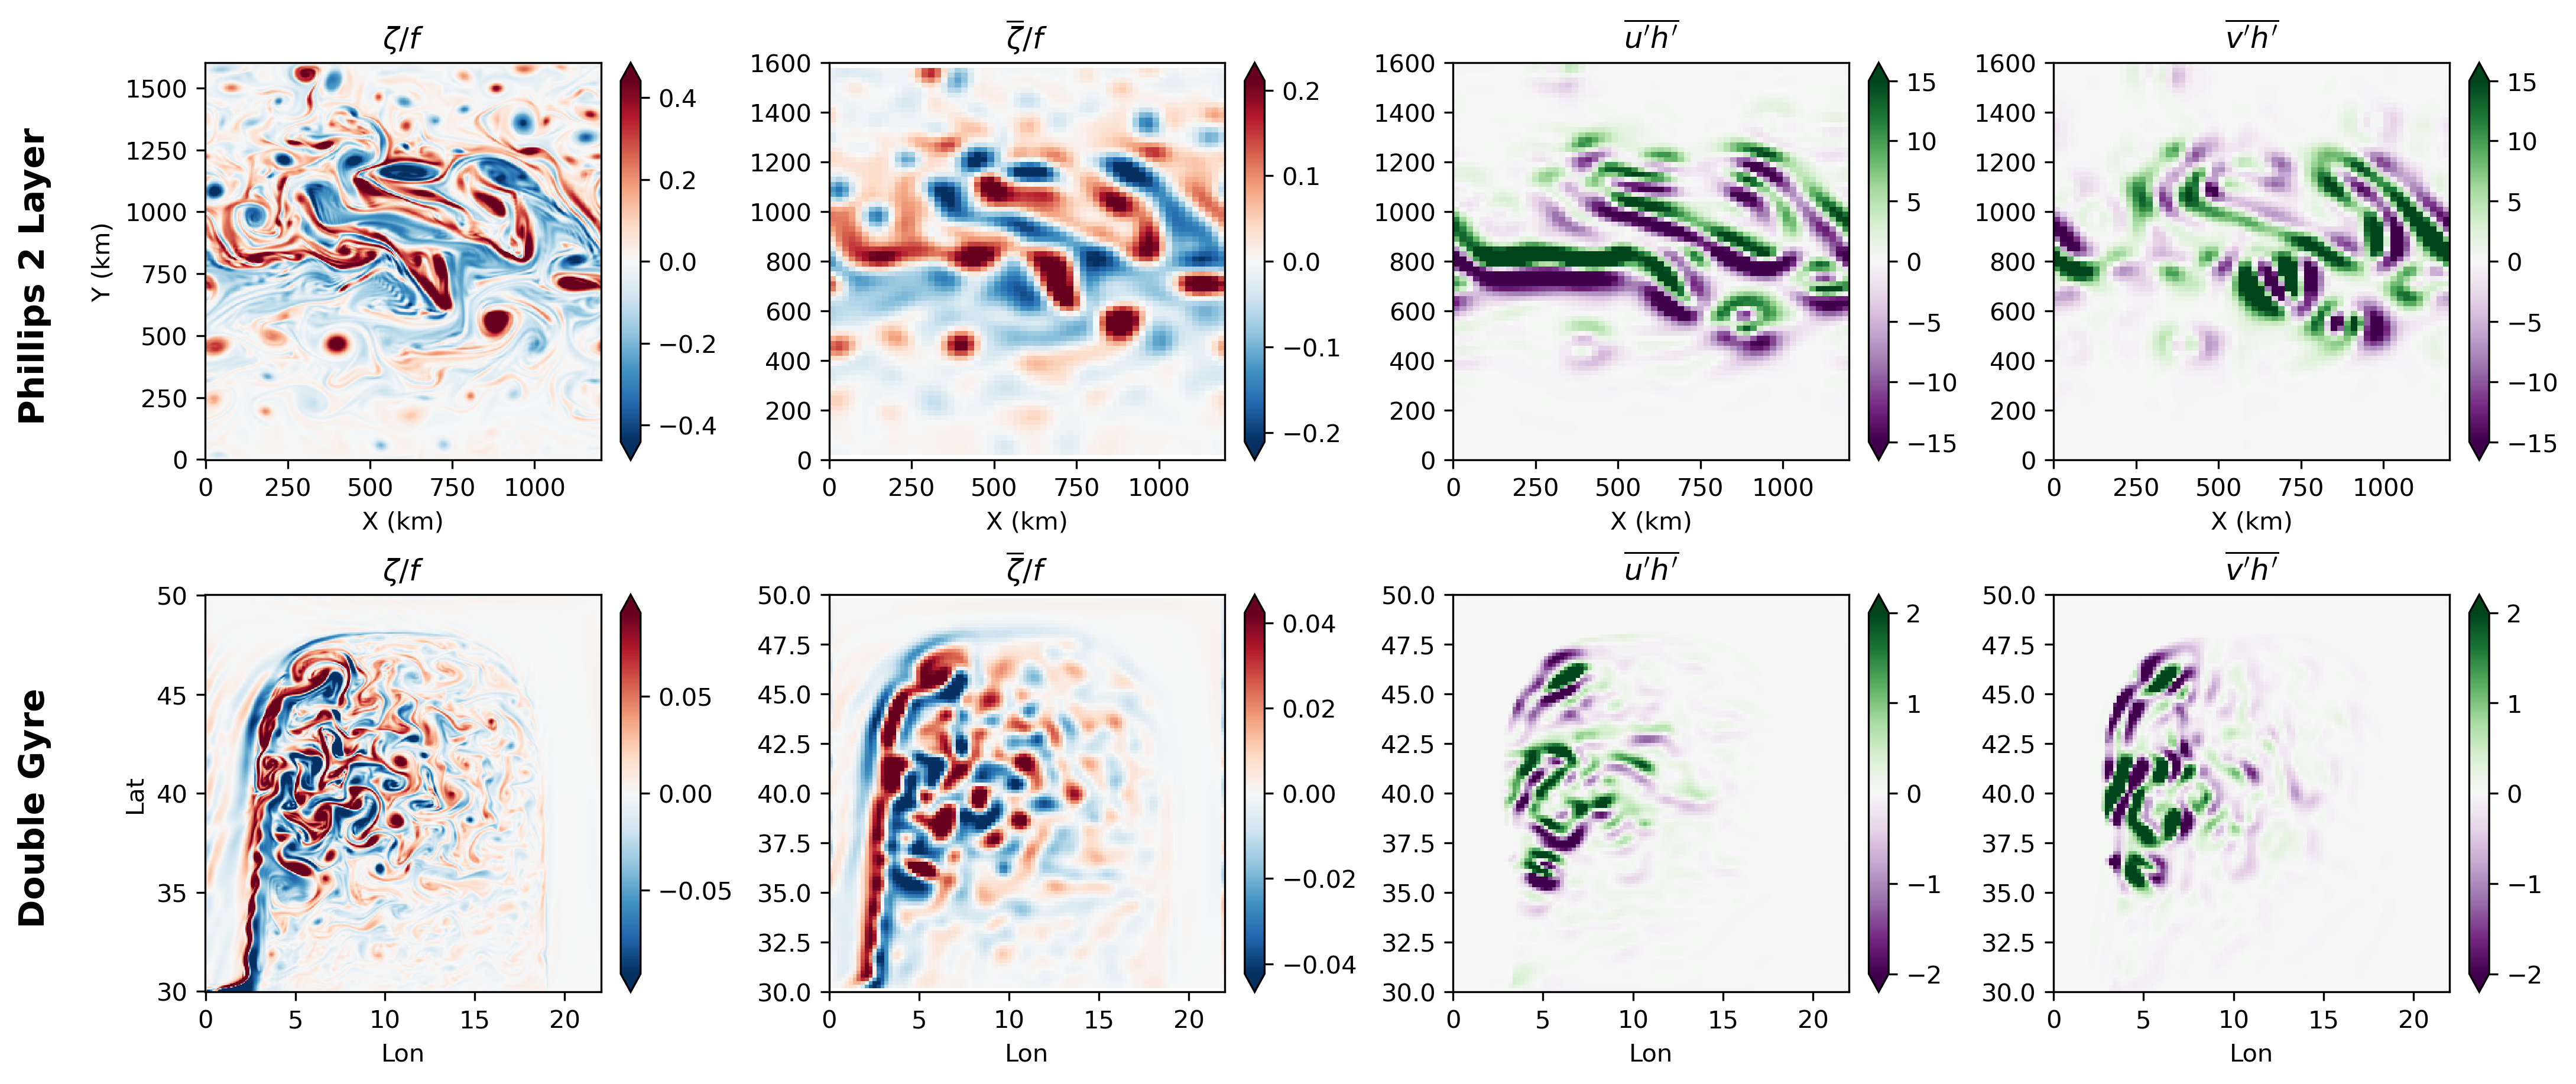
\includegraphics[width=\textwidth]{Figure1.png}
\caption{Snapshots exemplifying the high-resolution vorticity (left), filtered vorticity (second column), and sub-grid thickness fluxes (last two columns) from the Phillips 2 layer (top) and Double-Gyre (bottom). The filtered fields are shown from the case of coarse-graining scale of 20~km. Only the upper layer data is shown, and different panels have different color ranges. }
\label{fig:intro_panels}
\end{figure}


\begin{figure}
\noindent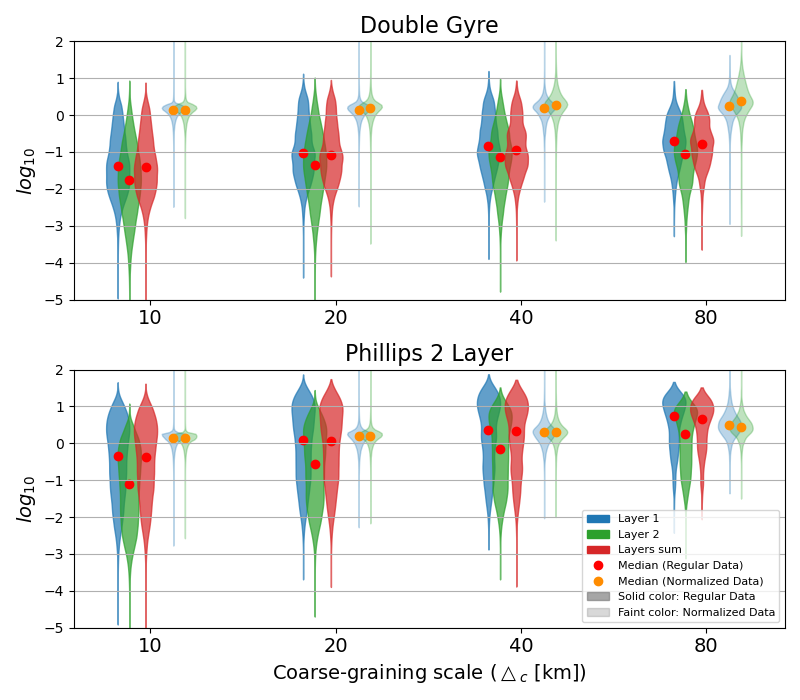
\includegraphics[width=\textwidth]{Figure2.png}
\caption{\textbf{Distribution of output data:} Distributions of the logarithm of the thickness flux magnitudes ($|\mathbf{F}_n|$) in both layers and their sum (barotropic contribution), and the normalized thickness flux ($\frac{|\mathbf{F}_n|}{\, \triangle_c^2 |\nabla \overline{\mathbf{u}}_n||\nabla \overline{h}_n|}$) in both layers for the different experiments (top and bottom panel) and different coarse-graining scales (indicated on the $x$-axis). The legend in the lower panel is used to indicate the different elements in both the panels. The density of the distribution is indicated by the width of each patch, with wider regions, usually in the middle, indicating a higher concentration of data points near those values.  }
\label{fig:dist_outputs}
\end{figure}

\begin{figure}
\noindent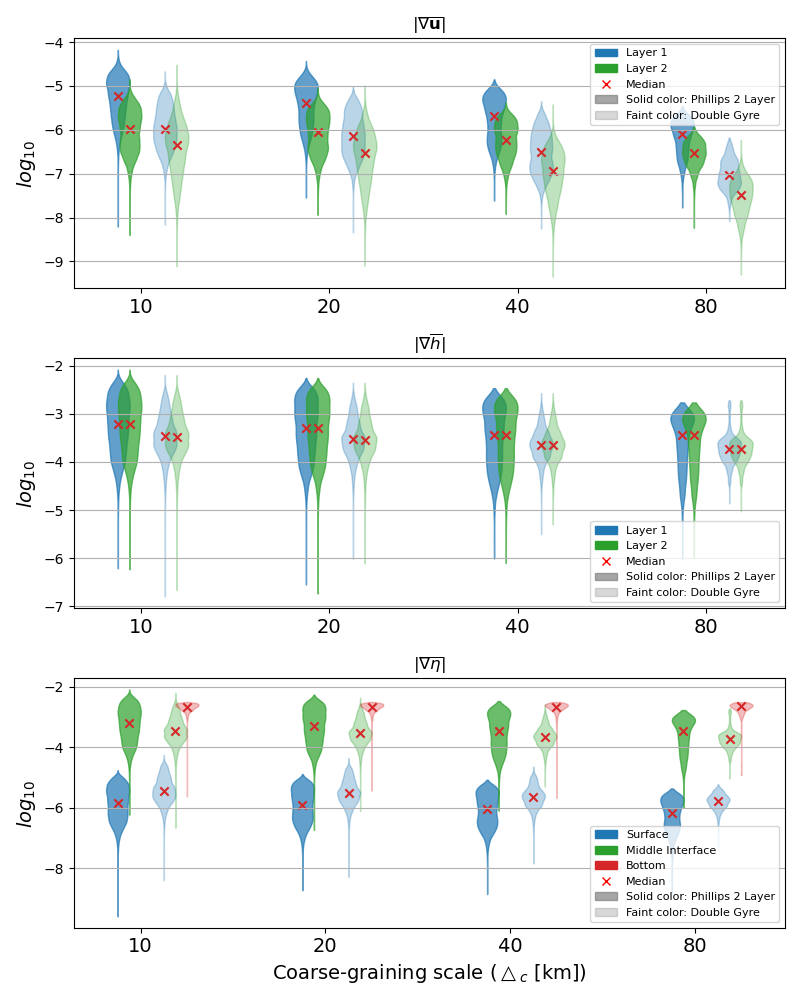
\includegraphics[width=\textwidth]{Figure3.png}
\caption{\textbf{Distribution of input data:} Distributions showing the logarithmic magnitude range of different filtered fields, which may be used as input variables for neural network design from both simulations and at different layers and interfaces. Similar to Figure \ref{fig:dist_outputs} the width of the patch corresponds to values with a higher probability of occurence.}
\label{fig:dist_inputs}
\end{figure}


\begin{figure}
\noindent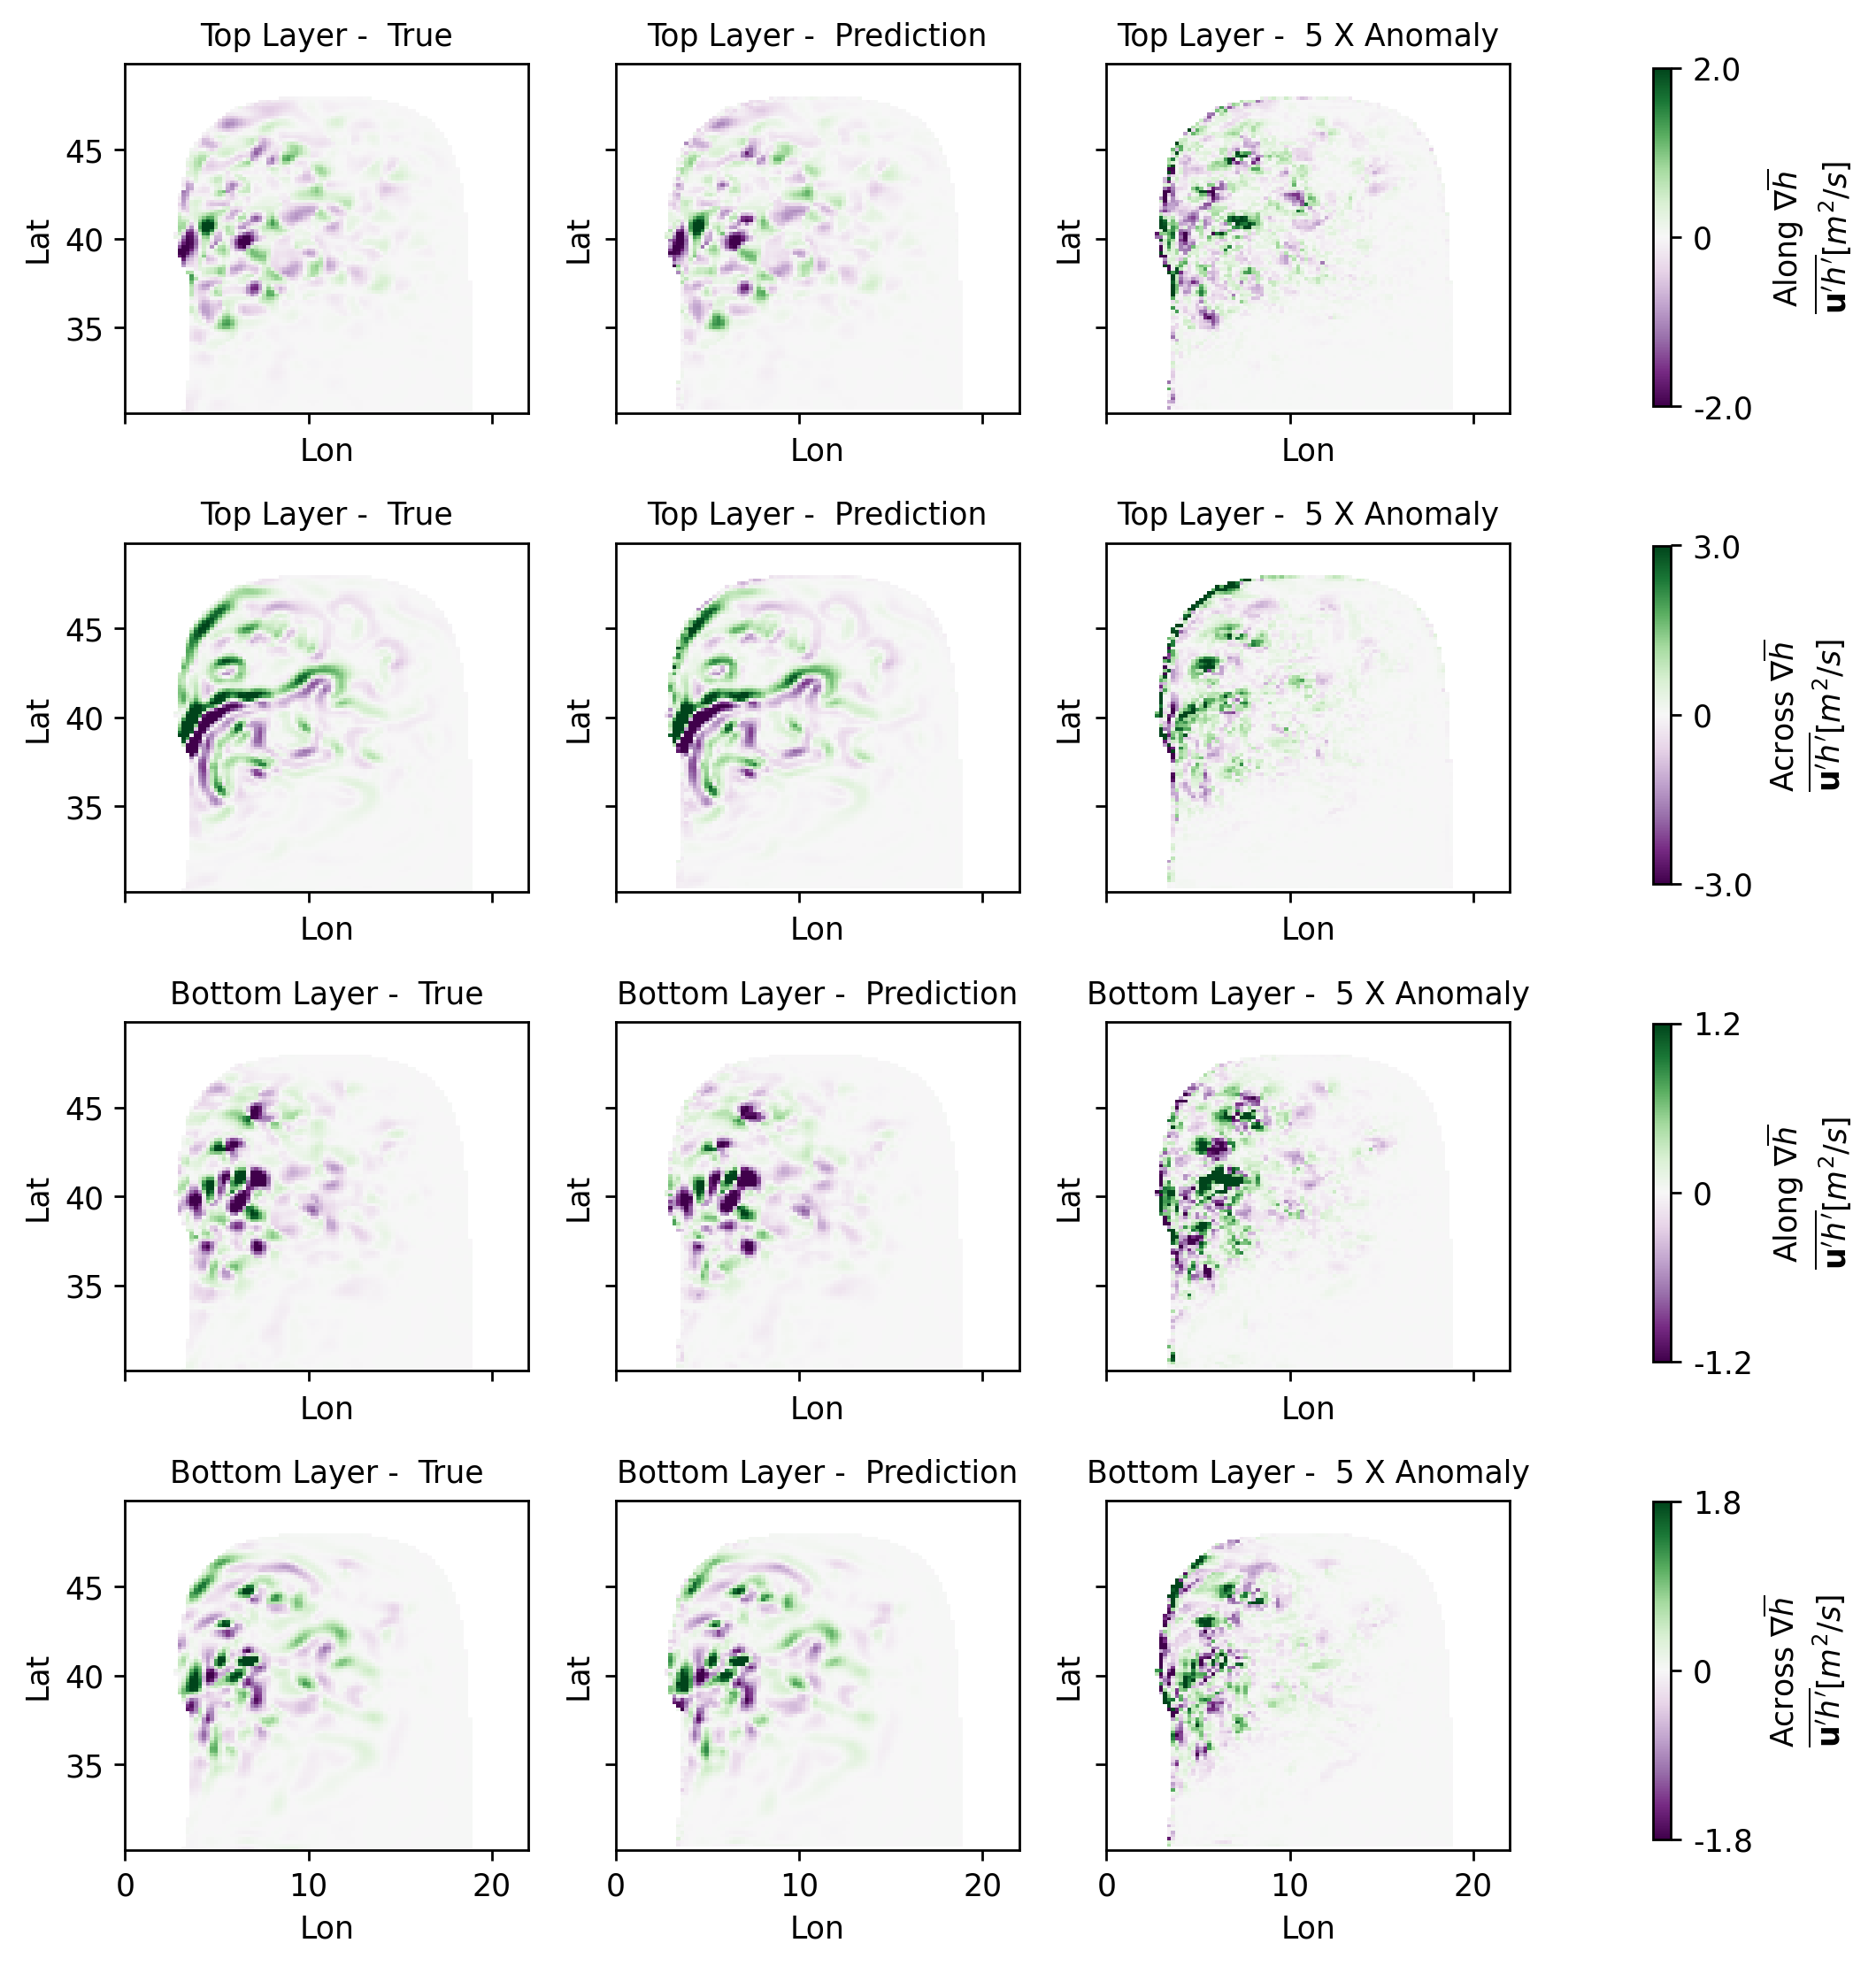
\includegraphics[width=\textwidth]{Figure4.png}
\caption{The true (1st column), predicted (2nd column), and prediction error (3rd column) in the along (1st and 3rd row) and across (2nd and 4th row) thickness gradient fluxes for the top (1st and 2nd row) and bottom (3rd and 4th row) layers of the Double-Gyre simulations. Here the results are shown for the ML model of the following configuration: $3\times3$ stencil, trained on data from Double-Gyre+Phillips-2-Layer, and $5090$ learnable parameters. These offline skill results are shown for the filter scale of $100$km. Note that the prediction error has been multiplied by a factor of 5 to be easily visible on the same scale as the true and predicted fluxes.}
\label{fig:poitwise_prediction_maps}
\end{figure}

\begin{figure}
\noindent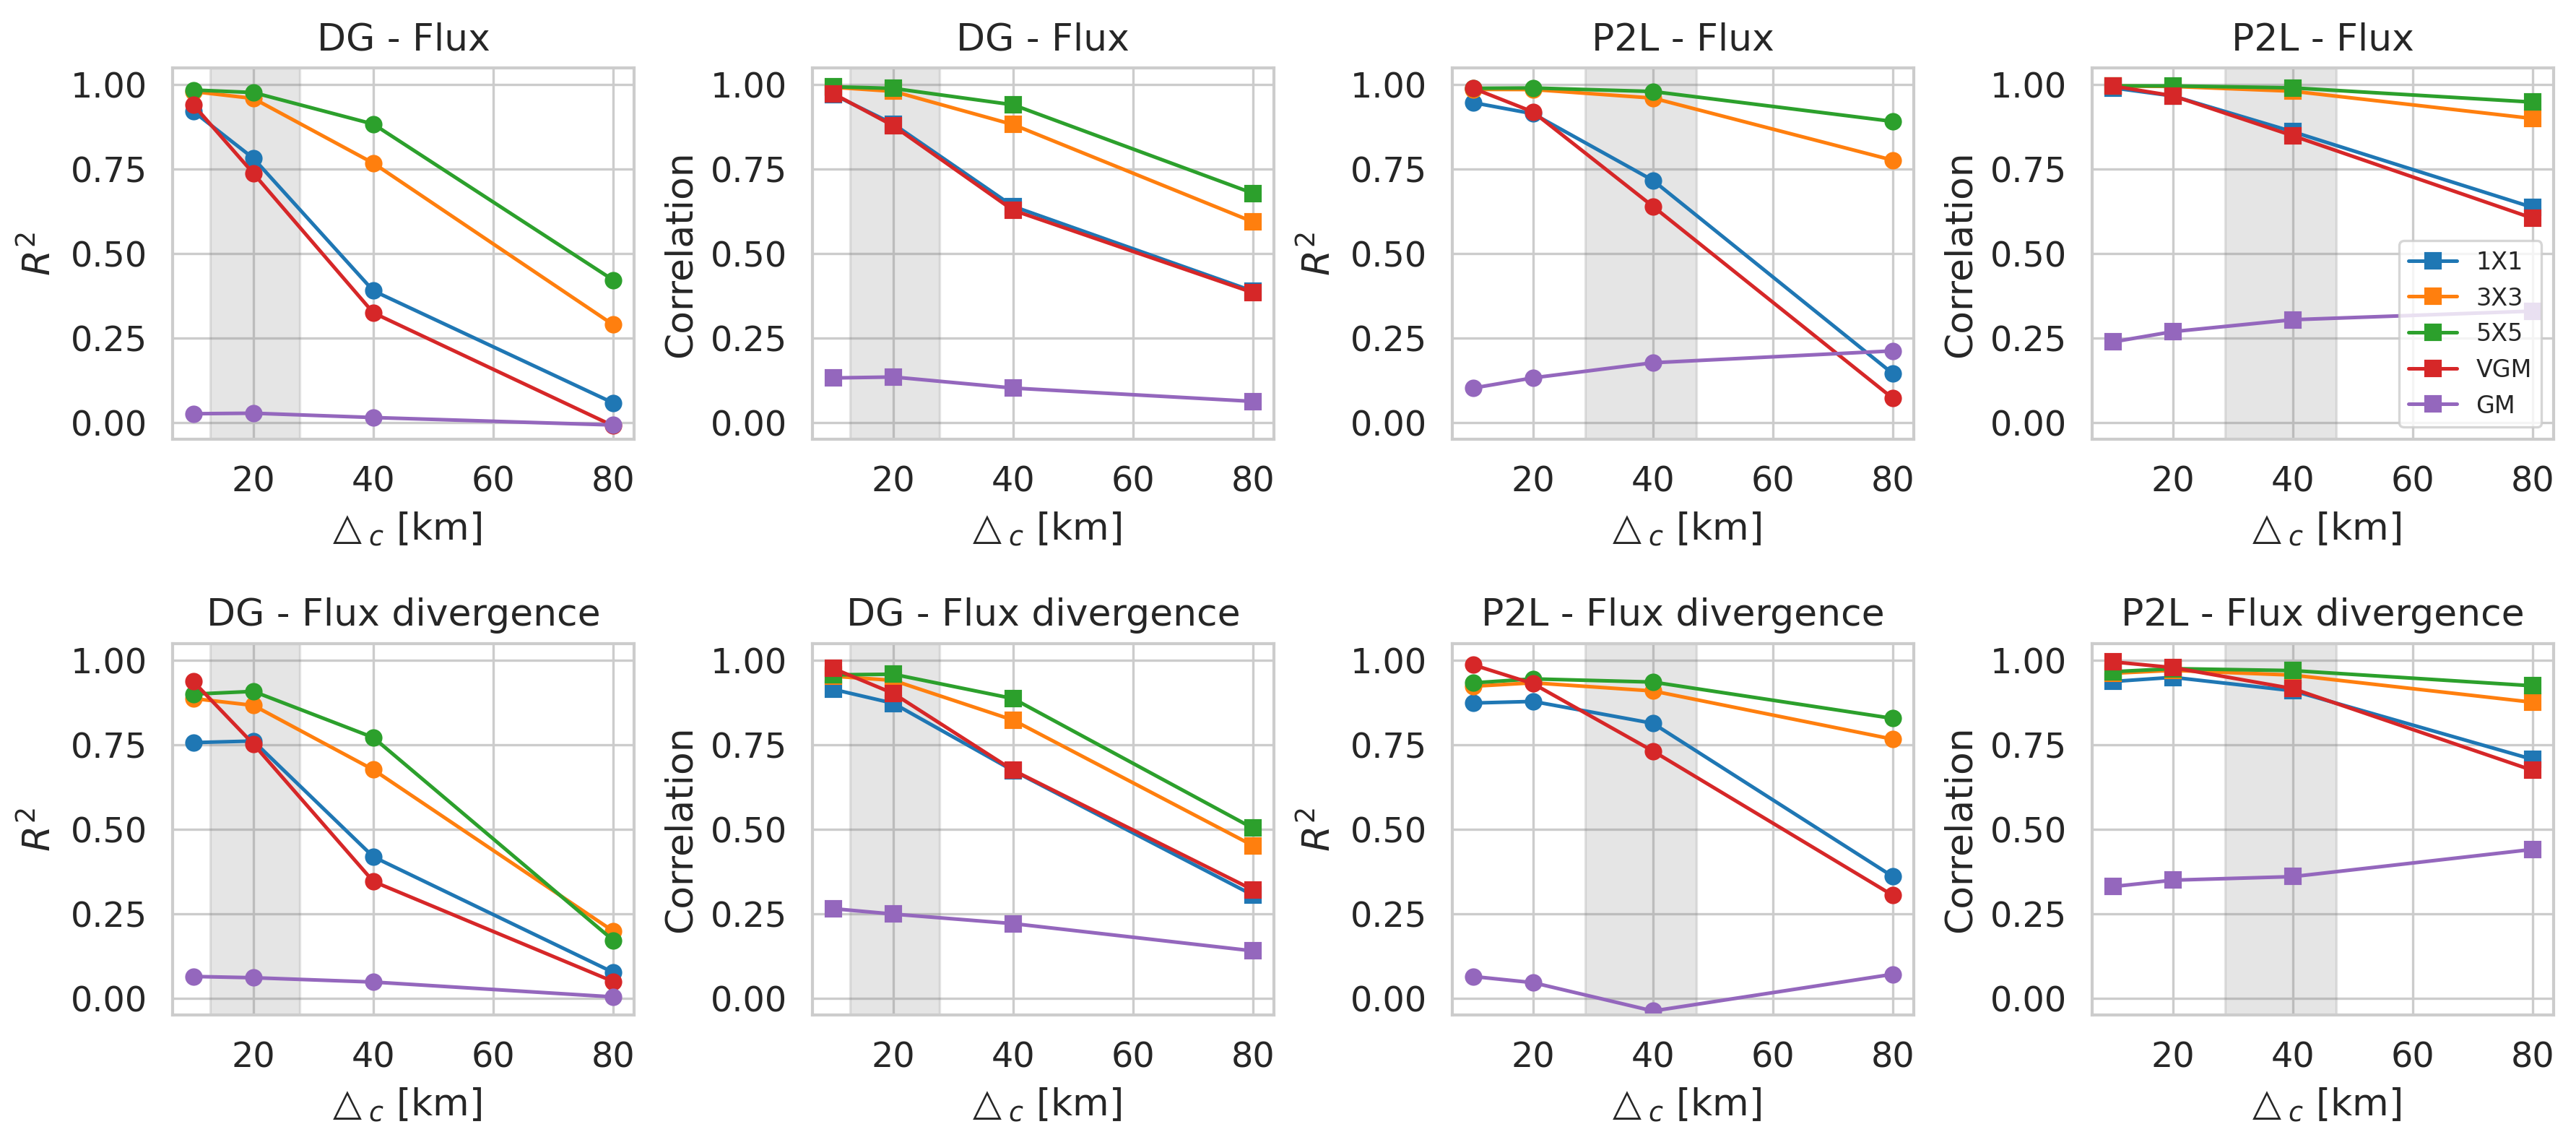
\includegraphics[width=\textwidth]{Figure5.png}
\caption{Pointwise offline skill in terms of the $R^2$ skill score (1st and 3rd columns) and correlation (2nd and 4th columns) for 5 different models (indicated in the legend) at different scales ($x$-axis) in the double gyre (1st and 2nd columns) and Phillips 2 layer (3rd and 4th columns) simulations. The top row shows skill for the sub-grid thickness flux and the bottom row shows skill for its divergence. The metrics were evaluated over the bottom layer and across the full test dataset spanning 33 years (1200 snapshots). The gray shaded area indicates the deformation radius range (10th to 90th percentile) in the simulation.}
\label{fig:pointwise_skill}
\end{figure}

\begin{figure}
\noindent\includegraphics[width=\textwidth]{Figure6.pdf}
\caption{Offline skill in predicting the time average of the subgrid thickness fluxes, using five different models (columns) for the Phillips-2-layer (P2L) and Double-Gyre (DG) simulations. 
For all models the skill in predicting the time averaged flux is quantified as the average skill over the two layers and for both the along and across thickness gradient direction. 
%For the Gent-McWilliams model the skill is taken as the average between the along and across thickness gradient fluxes. 
}
\label{fig:bulk_skill}
\end{figure}

\begin{figure}
    \centering
    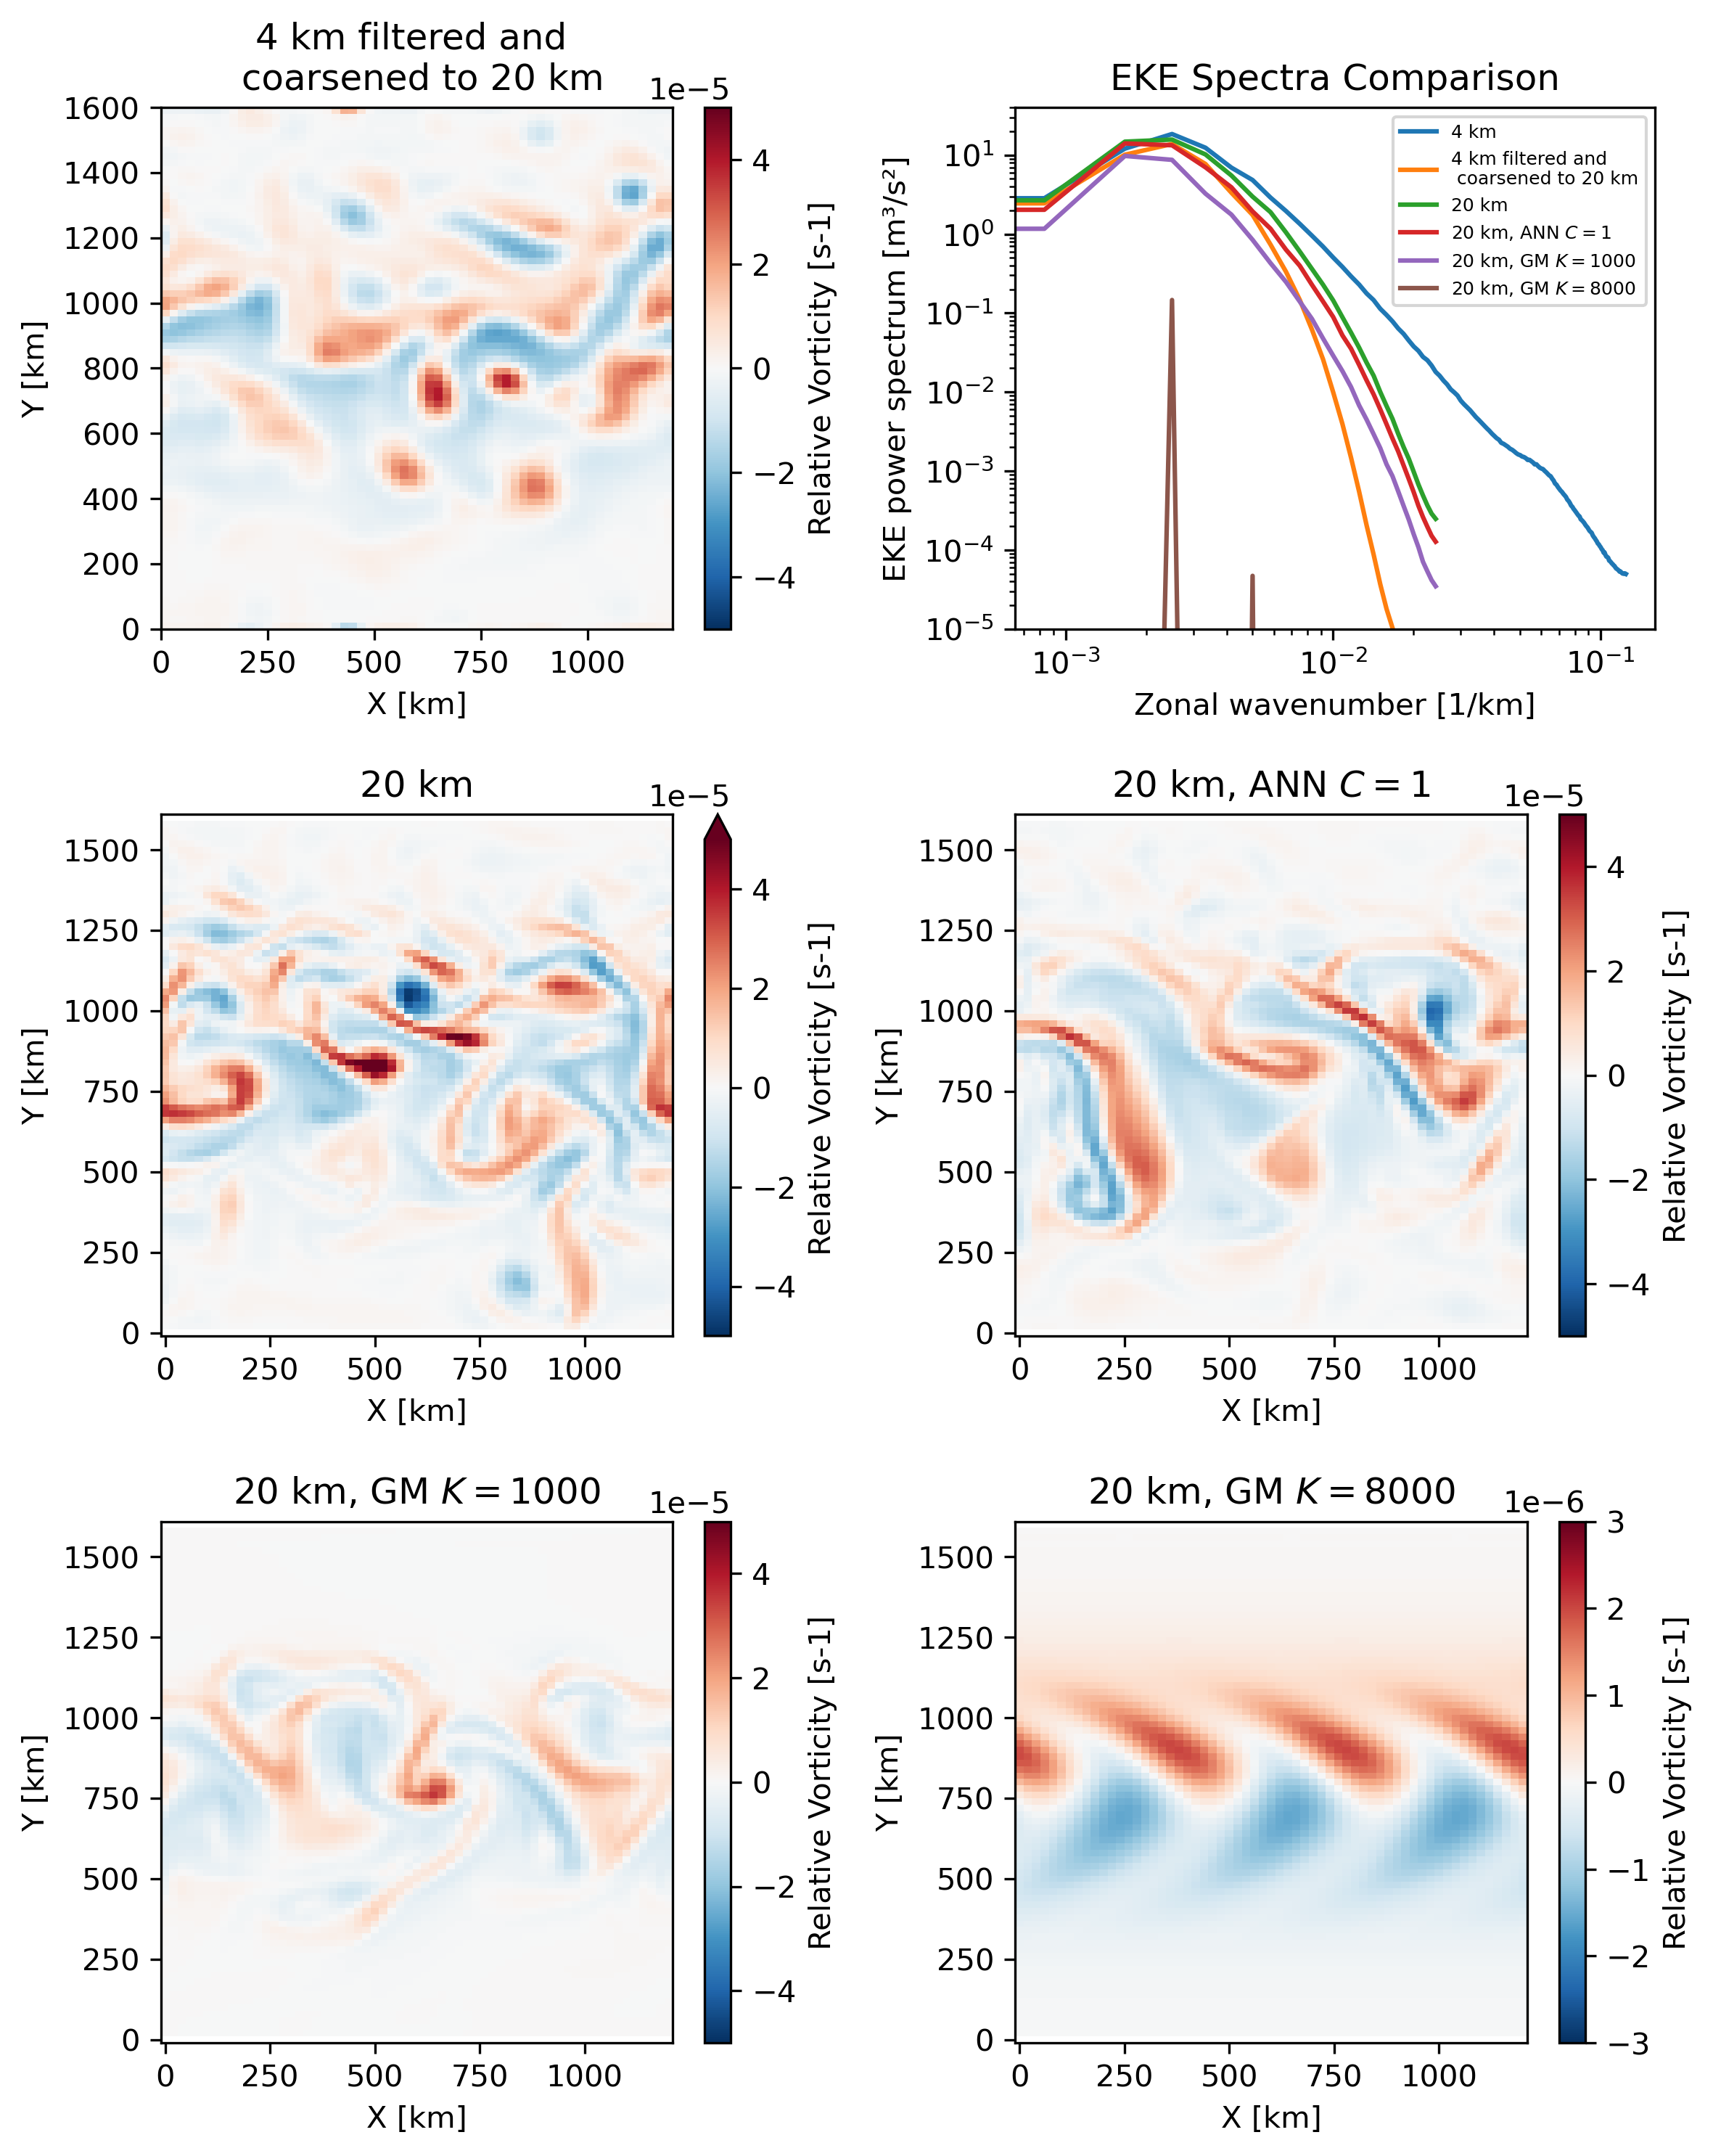
\includegraphics[width=\linewidth]{Figure7.png}
    \caption{Snapshots of relative vorticity and the EKE spectra from different Phillips 2 layer simulations discussed in section 4.2.
    Note that the colorbar on the bottom right panel has been adjusted to show the range of values in that simulation. }
    \label{fig:P2L_RV}
\end{figure}


\begin{figure}
    \centering
    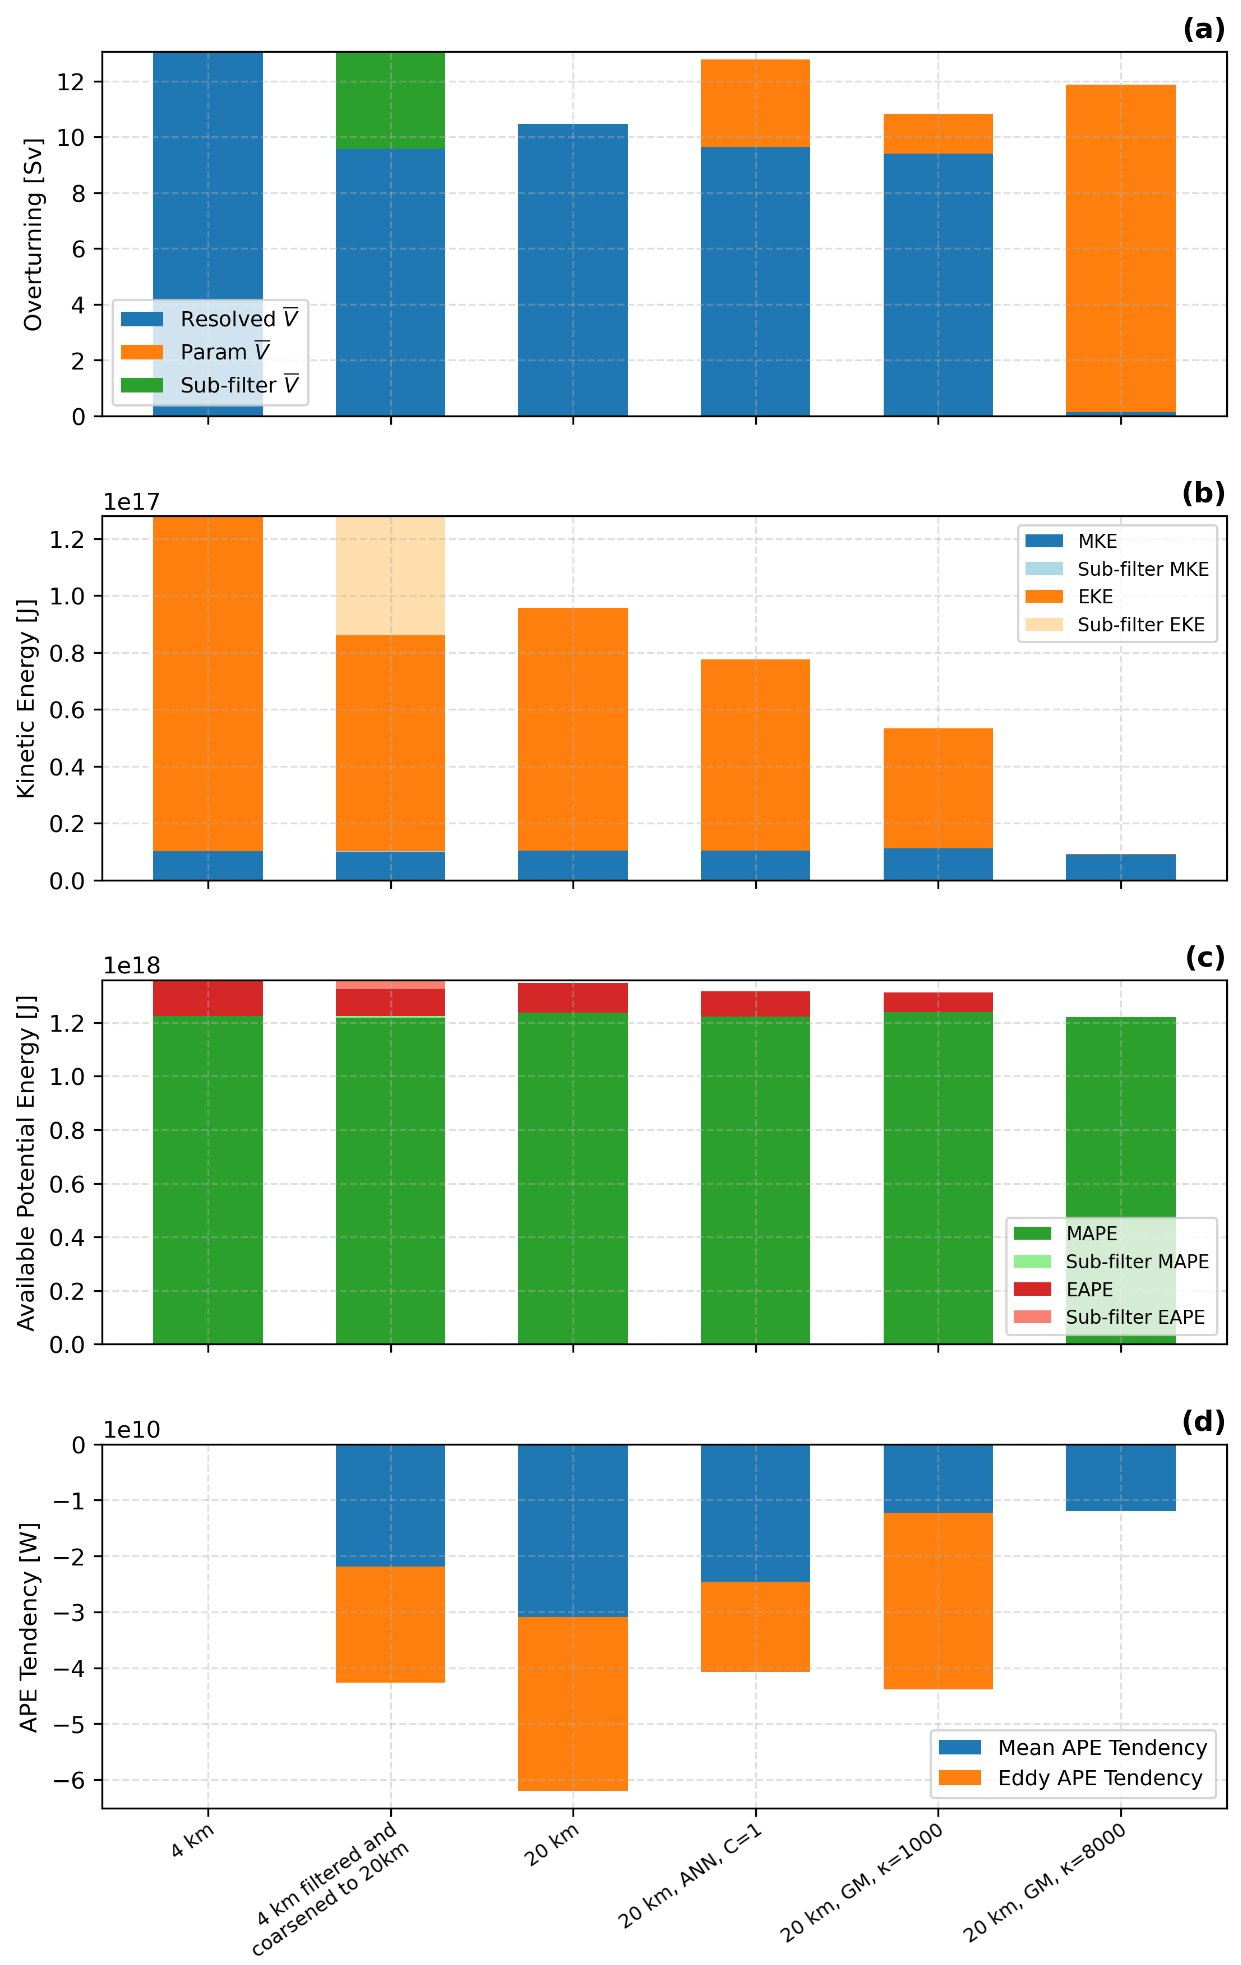
\includegraphics[width=0.8\linewidth]{Figure8.png}
    \caption{Bulk metrics to evaluate the online skill of the parameterizations in different experiments of Phillips 2 layer simulation (indicated along the $x$-axis). (a) Peak value of the total meridional transport in the upper layer for the resolved, parameterized and sub-filter components. (b) Kinetic energy and (c) available potential energy of the mean and eddy flow coming from the resolved and sub-grid contributions. (d) The impact of the parameterized or sub-grid thickness fluxes on the mean and eddy APE tendency; no bar plot is shown for the high-resolution simulation as in this instance there are no sub-grid or parameterized thickness flux, and the bar for the 20km simulation is calculated using sub-grid thickness fluxes predicted by a ANN that was not coupled with the resolved fields of the simulation.  }
    \label{fig:P2_all_panels}
\end{figure}



\begin{figure}
    \centering
    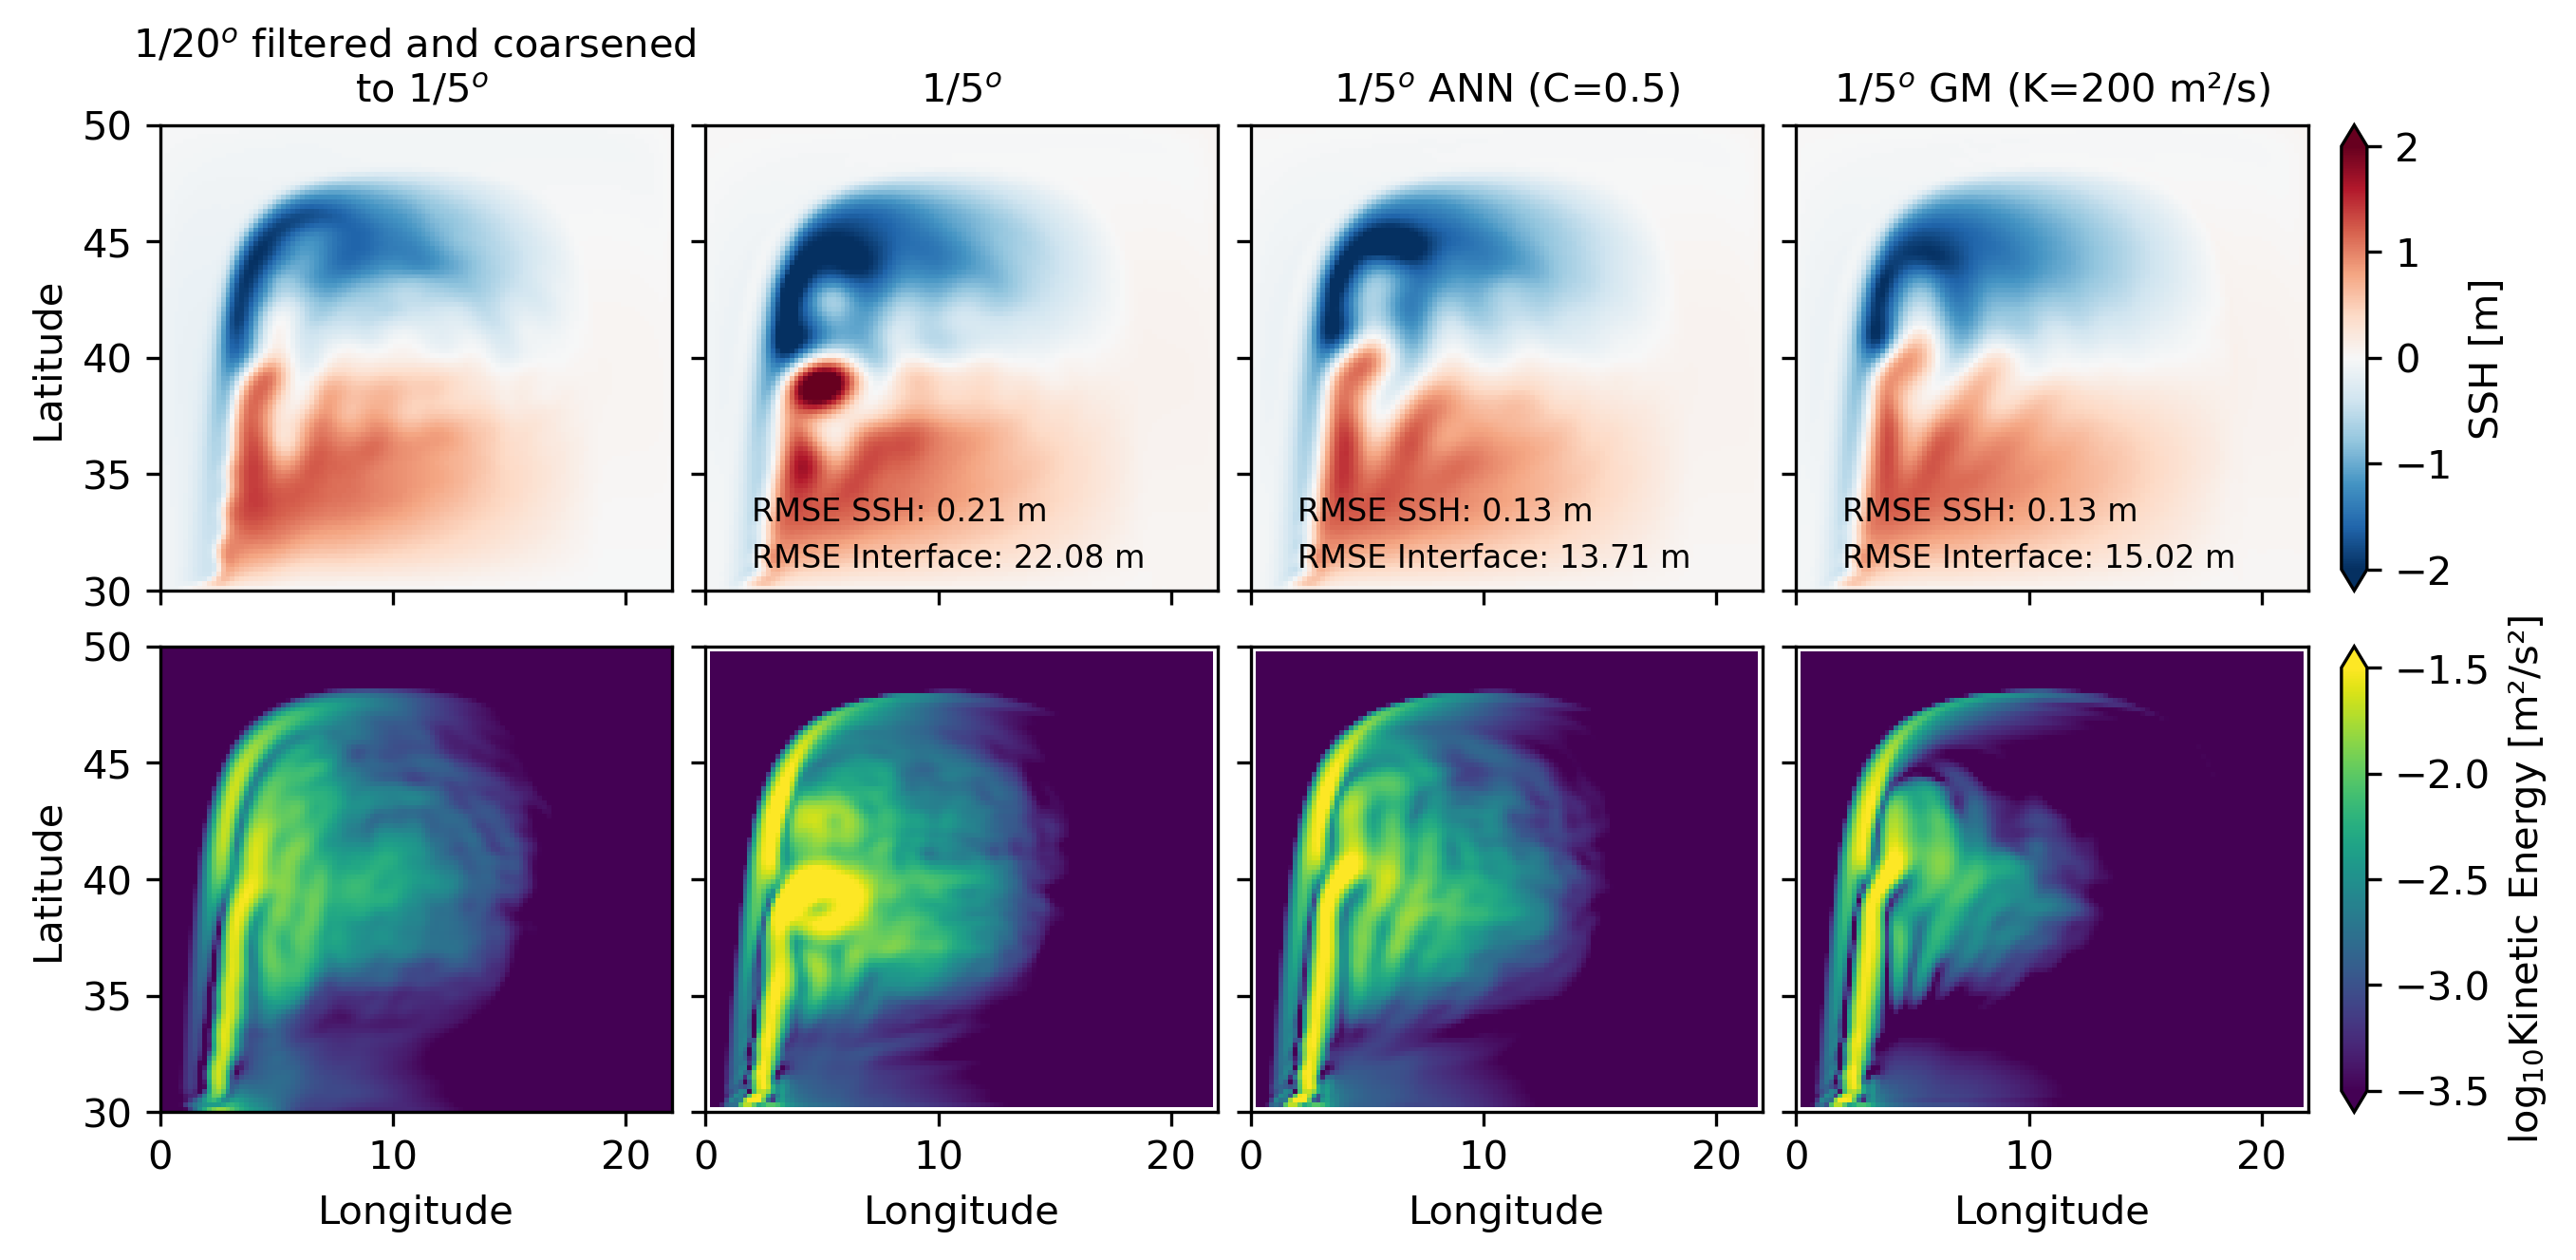
\includegraphics[width=\linewidth]{Figure9.png}
    \caption{Mean SSH (top row) and EKE (bottom row) the for the Double gyre simulations discussed in section 4.3. The RMSE in the SSH and middle interface height are indicated for the three $1/5^\circ$ resolution simulations.}
    \label{fig:DG_maps}
\end{figure}
  
\begin{figure}
    \centering
    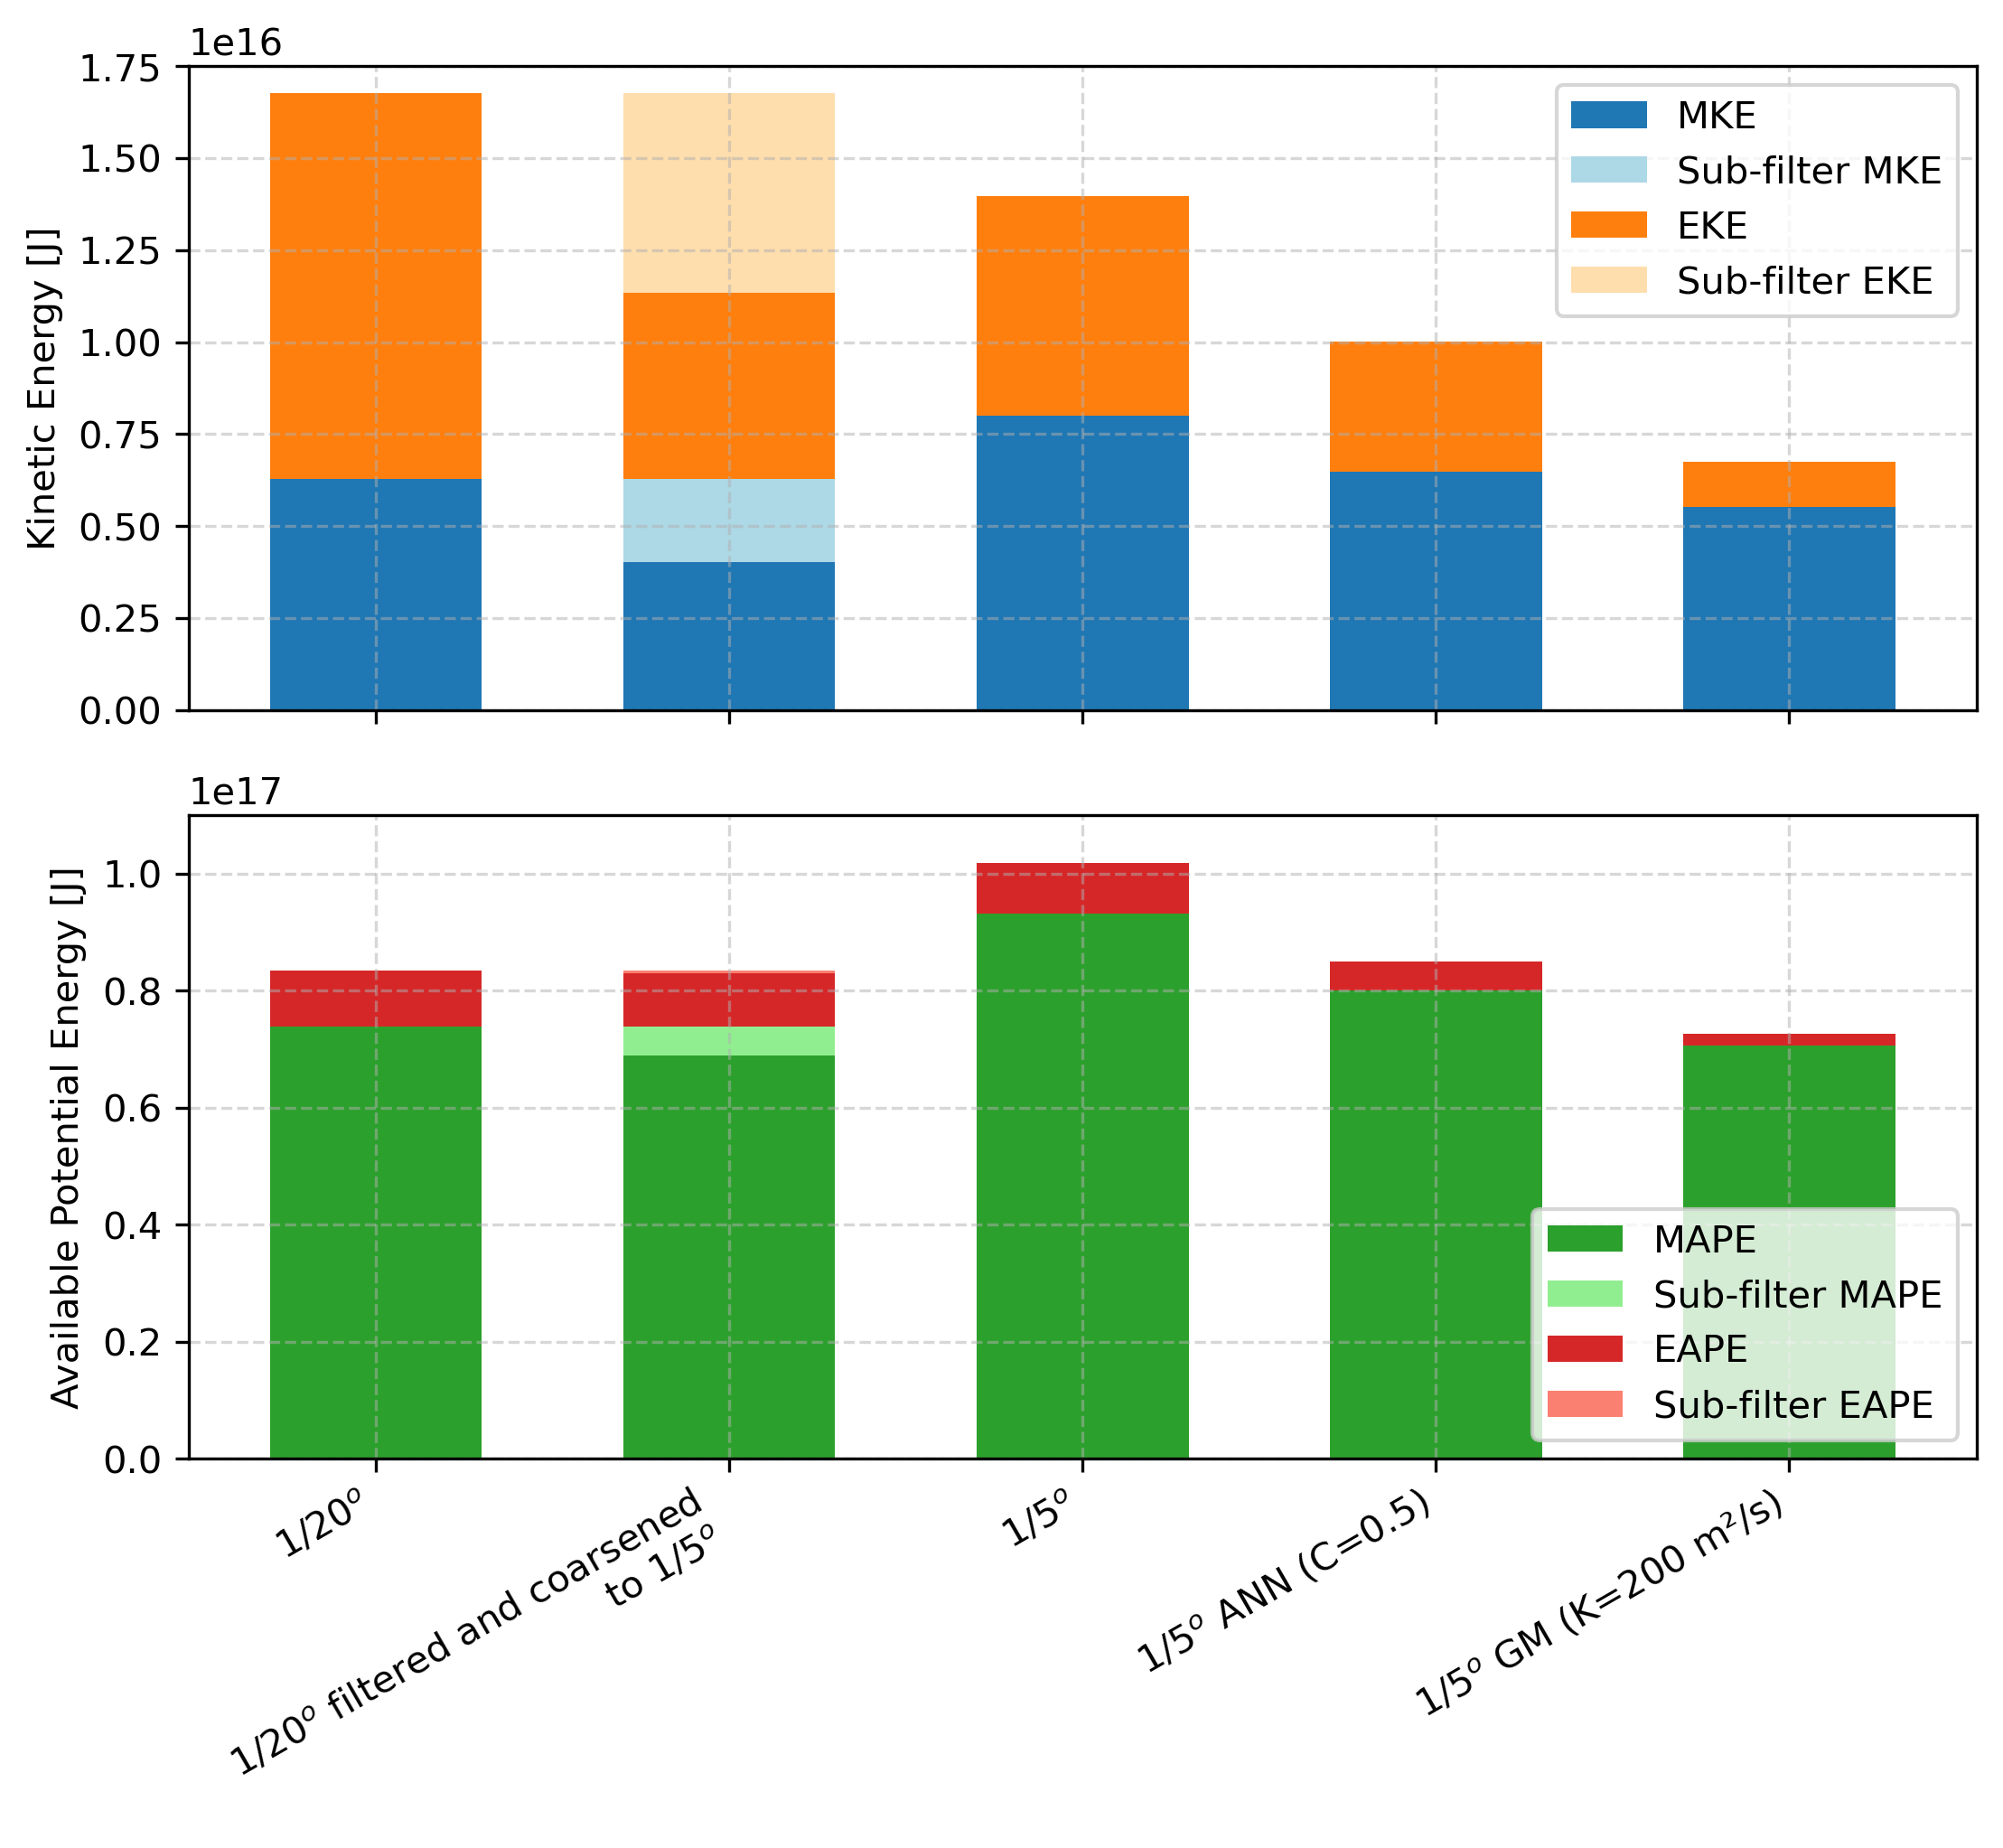
\includegraphics[width=0.9\linewidth]{Figure10.png}
    \caption{The volume integrated KE (top) and APE (bottom) for the Double-Gyre simulations (indicated along $x$-axis) discussed in section 4.3. The mean, eddy, and sub-filter contributions are indicated. }
    \label{fig:DG_energy}
\end{figure}

\begin{figure}
    \centering
    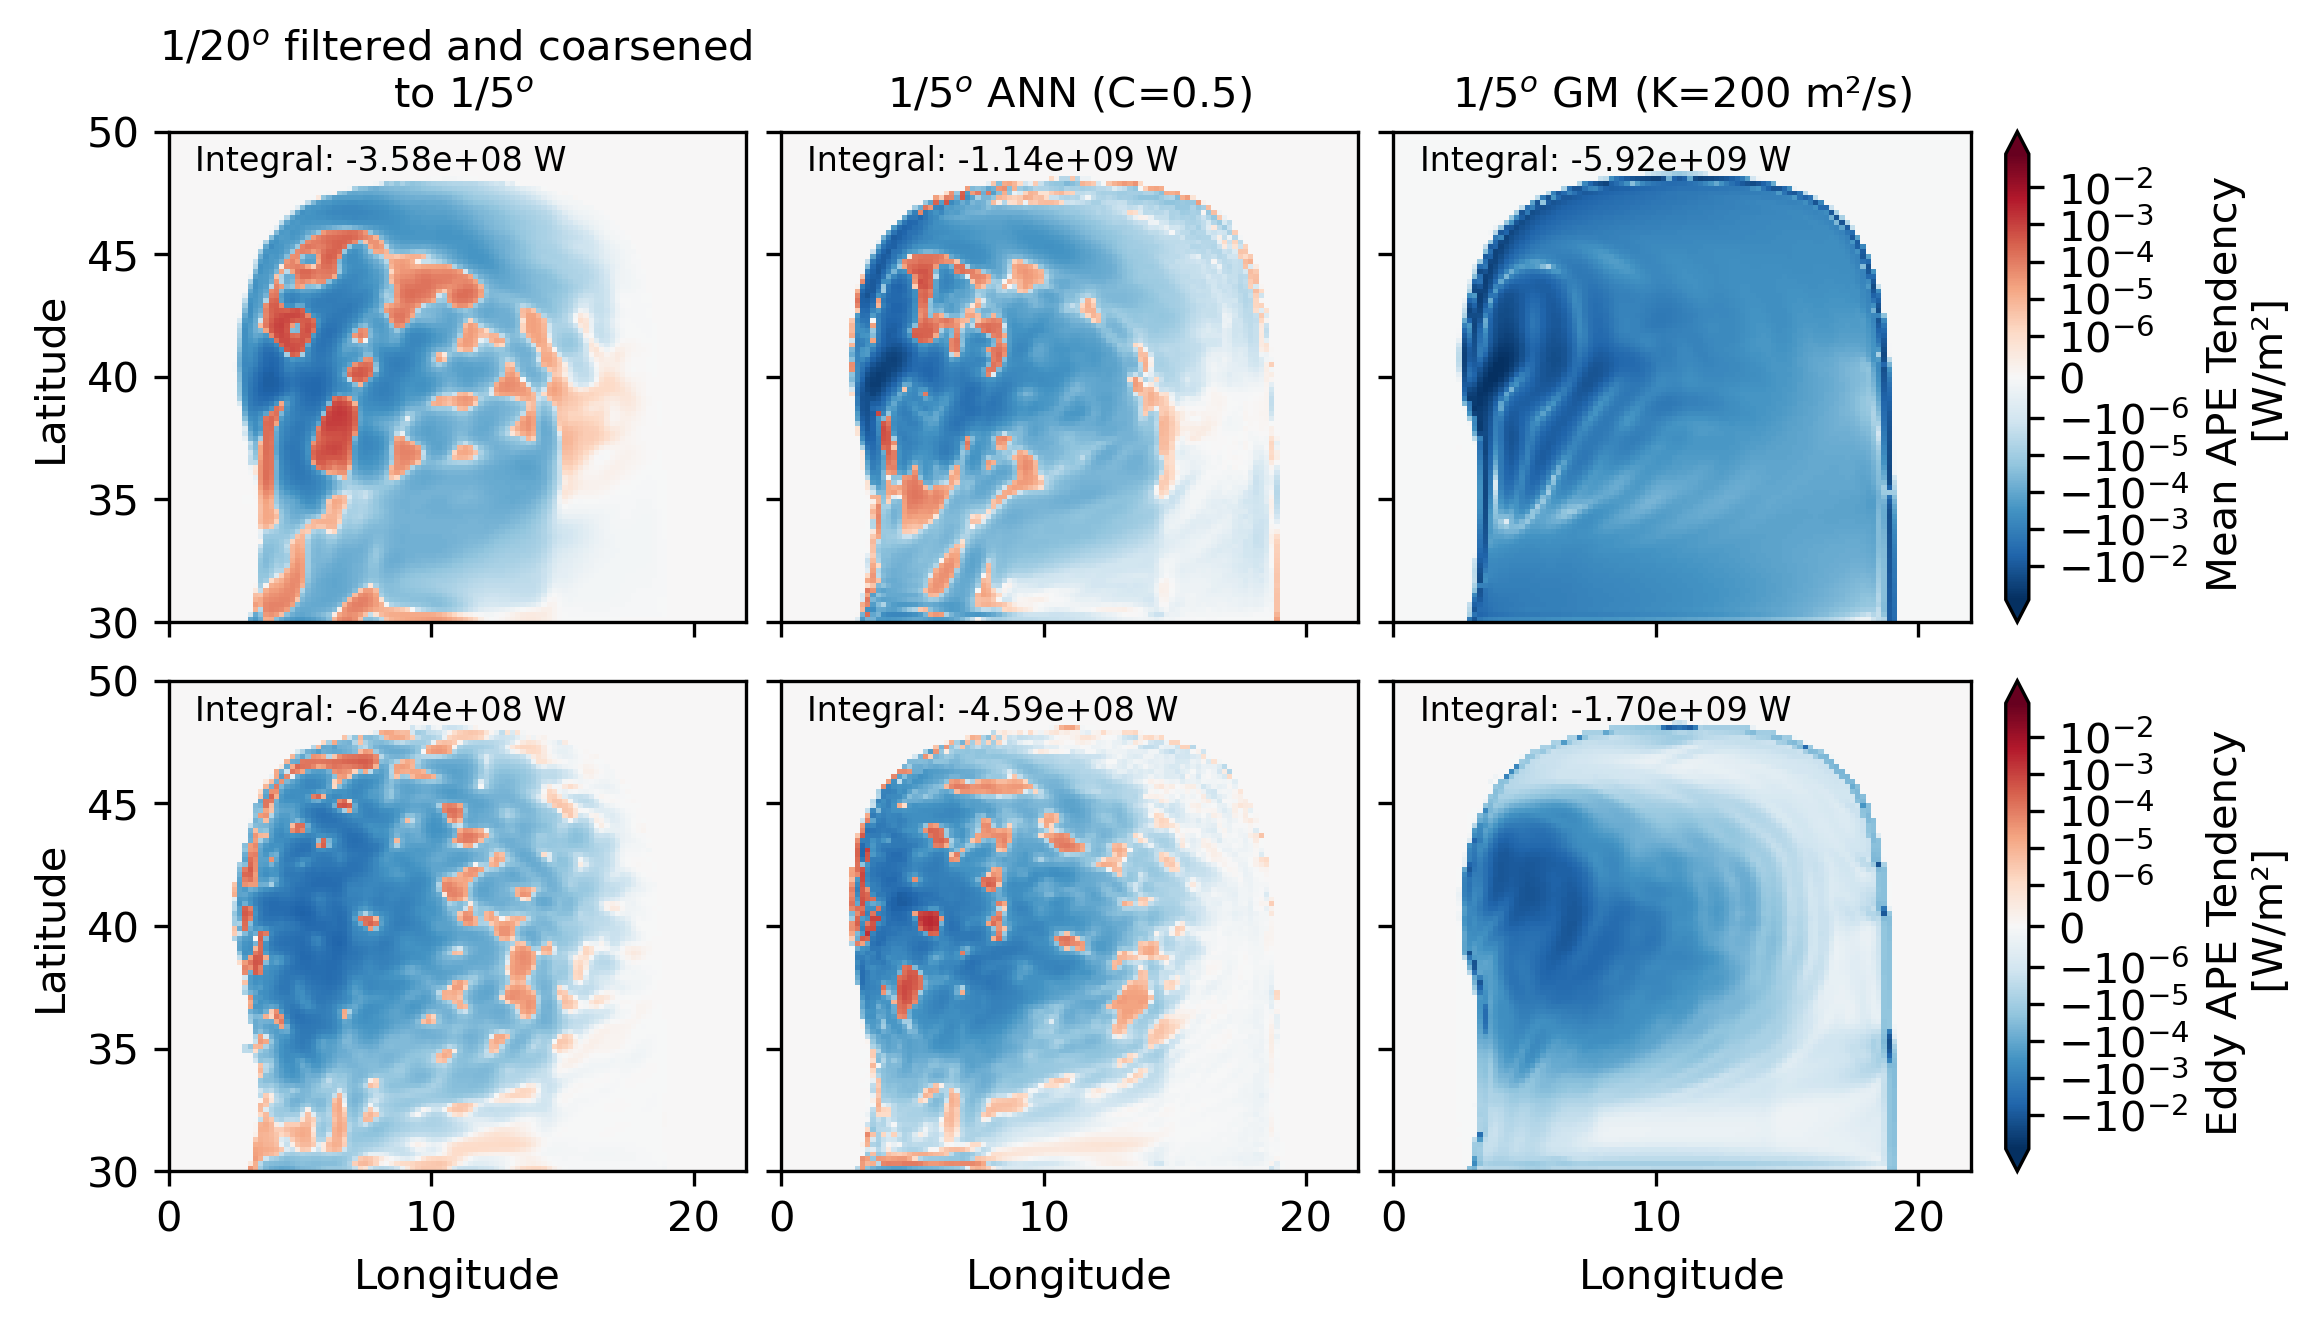
\includegraphics[width=\linewidth]{Figure11.png}
    \caption{APE tendency exerted on the mean (top) and eddy (bottom) APE by the sub-grid or parameterized fluxes in the Double-Gyre simulations discussed in section 4.3. The volume integrated value for each panel is indicated at the top left.  }
    \label{fig:DG_APE_tend}
\end{figure}

%%%%%%%%%%%%%%%%%%%%
%%%% Appendix %%%%%%%
%%%%%%%%%%%%%%%%%%%%



\bibliography{references}

\end{document}
